\documentclass[10pt,a4paper]{article}

% ---------------------------------------------------------------------------
% Typography: ML-conference look (Computer Modern), with full Cyrillic.
%
% Latin Modern has no Cyrillic coverage, so the body font is Computer Modern
% Unicode (cm-unicode), loaded by path because it is shipped with TeX Live but
% not registered with fontconfig under a friendly name. Math stays Latin Modern
% Math, which is metrically the same design, so symbols and body text agree.
% This is a visually close academic style, NOT the official ICLR style package,
% and the document carries no conference branding.
% ---------------------------------------------------------------------------
\usepackage{fontspec}
\usepackage{unicode-math}

\newcommand{\cmupath}{/usr/share/texlive/texmf-dist/fonts/opentype/public/cm-unicode/}
\setmainfont{cmunrm.otf}[Path=\cmupath,
  BoldFont=cmunbx.otf, ItalicFont=cmunti.otf, BoldItalicFont=cmunbi.otf]
\setsansfont{cmunss.otf}[Path=\cmupath,
  BoldFont=cmunsx.otf, ItalicFont=cmunsi.otf]
\setmonofont{cmuntt.otf}[Path=\cmupath,
  BoldFont=cmuntb.otf, ItalicFont=cmunit.otf, Scale=0.94]
\setmathfont{Latin Modern Math}

\usepackage{polyglossia}
\setmainlanguage{russian}
\setotherlanguage{english}

% Conference-paper density: one column (the Pareto figures and mechanistic
% tables are wide and would suffer in two), but a tighter measure and leading
% than a default article.
\usepackage[a4paper,top=2.5cm,bottom=2.6cm,left=2.7cm,right=2.7cm]{geometry}
\linespread{1.04}
% lines dense with unbreakable \texttt tokens would otherwise overhang the margin
\emergencystretch=1.6em

\usepackage{amsmath}
\usepackage{graphicx}
\usepackage{booktabs}
\usepackage{array}
\usepackage[font=small,labelfont=bf,labelsep=colon,skip=6pt]{caption}
\usepackage{float}
\usepackage[table]{xcolor}
\usepackage[hidelinks,breaklinks]{hyperref}
\usepackage{enumitem}
\usepackage{tcolorbox}
\usepackage{titlesec}
\usepackage{titletoc}
\usepackage{microtype}

\definecolor{accent}{HTML}{1F5FA8}
\definecolor{neg}{HTML}{A6432E}
\definecolor{inksoft}{HTML}{48596B}
\definecolor{rulegrey}{HTML}{C4CDD7}

% Compact bold headings in the conference-paper idiom, not oversized ones.
\titleformat{\section}{\normalfont\large\bfseries}{\thesection}{0.7em}{}
\titleformat{\subsection}{\normalfont\normalsize\bfseries}{\thesubsection}{0.6em}{}
\titlespacing*{\section}{0pt}{2.2ex plus .6ex minus .2ex}{1.1ex plus .2ex}
\titlespacing*{\subsection}{0pt}{1.8ex plus .5ex minus .2ex}{0.8ex plus .2ex}

% TOC: explicit number widths so the number never abuts the title.
\titlecontents{section}[1.9em]{\vspace{1.8pt}}
  {\contentslabel{1.9em}}{\hspace*{-1.9em}}
  {\hspace{0.5em}\titlerule*[0.7pc]{.}\contentspage}
\titlecontents{subsection}[4.3em]{}
  {\contentslabel{2.5em}}{\hspace*{-2.5em}}
  {\hspace{0.5em}\titlerule*[0.7pc]{.}\contentspage}

\captionsetup[figure]{name=Рис.}
\captionsetup[table]{name=Таблица}
\setlist{noitemsep,topsep=3pt,parsep=1pt}
\renewcommand{\arraystretch}{1.08}

% Shorthands for the geometry this report is about. Using math mode here is not
% cosmetic: an earlier Markdown build lost two table cells because the parallel
% and perpendicular norms were written with literal pipe characters, which the
% table parser read as column separators.
% SHA-256 digests are single unbreakable words; seqsplit lets them wrap in tables
\usepackage{seqsplit}
\newcommand{\shafull}[1]{\texttt{\seqsplit{#1}}}
\newcommand{\dhpar}{\lVert \Delta h_{\parallel} \rVert}
\newcommand{\dhperp}{\lVert \Delta h_{\perp} \rVert}
\newcommand{\ahat}{\hat{\alpha}}

\title{\vspace{-1.4cm}\bfseries Дешёвые обучаемые методы коррекции\ активаций для стиринга:\\ результаты}
\author{}
\date{}

\begin{document}

\begin{center}
{\LARGE\bfseries
Дешёвые обучаемые методы коррекции\ активаций для стиринга:\\ результаты
\par}

\vspace{0.9em}

{\small
GPT-2 small, точка вмешательства
\texttt{blocks.7.hook\_resid\_pre}, направления из SAE.
\par}

\vspace{0.75em}
\end{center}

\begin{tcolorbox}[colback=white,colframe=accent,boxrule=0.9pt,arc=1pt,
                  left=10pt,right=10pt,top=8pt,bottom=8pt]
\textbf{\large Краткое резюме}\medskip

\textbf{Задача.} Уменьшить негативный эффект стиринга активаций, сохранив или
усилив нужное свойство текста.

\textbf{Базовый компромисс.} Обычный аддитивный стиринг $h + \alpha v$ задаёт
выраженный компромисс: качество монотонно падает с ростом $\ahat$, а активация
целевой SAE-фичи достигает пика около $\ahat \approx 0.4$--$0.5$ и затем
обрушивается. Лексиконная метрика при экстремальном стиринге может при этом
\emph{ложно расти} за счёт деградации текста (\S\ref{sec:additive}).

\textbf{Что проверено.} Предложенный в задании гауссов денойзер действительно
решает свою вспомогательную задачу — убирает 32--57\,\% ущерба от гауссова
повреждения активаций. Но выигрыш на стиринге воспроизводится обычным скалярным
сжатием $\kappa = 0.8$, то есть является ослаблением стиринга, а не
исправлением активации. Дальше последовательно проверены: недостаточная ёмкость
модели (для варианта с обычным шумом увеличение размера с $16\text{M}$ до
$60\text{M}$ улучшило реконструкцию на 14.5\,\%, но не дало выигрыша в стиринге),
отсутствие информации о целевой координате и возможность получить номинальный
выигрыш за счёт изменения самой целевой координаты
(жёсткий клэмп закрыл лазейку и оказался сильным бейзлайном ценой
$+0.003\ldots+0.054$ ната), и наконец различие между шумом при обучении и ограничением при применении.

\textbf{Итог.} Модель с ортогональным шумом уверенно решает свою задачу
(T1: восстановлено 77.3\,\%), но при точно зафиксированной координате делает
качество \emph{хуже} жёсткого клэмпа (T2: $\Delta\mathrm{NLL} = +0.006184$,
95\,\% ДИ $[+0.001631, +0.010788]$; ни одна из 30 дополнительных конфигураций не дала улучшения).

\medskip
\textbf{Умение восстанавливать естественные активации само по себе не
переносится на исправление искажений, возникающих при стиринге.} Ущерб монотонно растёт вместе
с нормой ортогональной коррекции, а простой жёсткий клэмп остаётся более сильным
бейзлайном в исследованном режиме.

\smallskip
{\small Выполнены четыре дополнительных проверки (\S\ref{sec:poststop}):
геометрия пути повреждения (A) и обучение прямо на стиринг-подобном повреждении
(B) воспроизводят тот же отрицательный результат; условные средние естественных
активаций нелинейно зависят от выбранной линейной координаты, но этот эффект не
специфичен для концептных направлений (C); положительный контроль на заведомо
причинном направлении (D) показывает, что геометрия выравнивания не является
критерием управляемости.}
\end{tcolorbox}

\vspace{0.35cm}

\begin{center}
\small
\begin{tabular}{@{}ll@{}}
\textbf{Веса} & \url{https://huggingface.co/qweclownq/steering-denoisers}\\
\textbf{Финальная модель} & \url{https://huggingface.co/qweclownq/tangent-flow-16m}\\
\textbf{Репозиторий} & \url{https://github.com/zxclwnq/steering-denoisers}\\
\end{tabular}

\end{center}

\vfill

\clearpage
\tableofcontents
\clearpage

%==============================================================================
\section{Постановка задачи}

Стандартный аддитивный стиринг \cite{turner2023actadd,li2023iti} заменяет
активацию остаточного потока
\[
  \tilde h = h + \alpha v ,
\]
где $v$ — направление концепта, полученное из разреженного автоэнкодера
\cite{bricken2023monosemanticity,gao2024scalingsae}. Рост $\alpha$ усиливает
выражение концепта, но портит поведение модели. Интересен поэтому не уровень
качества и не сила концепта по отдельности, а \textbf{фронт Парето между ними}.

«Улучшить стиринг» означает строго одно из двух:
\begin{itemize}
  \item более сильный концепт при том же качестве, \textbf{или}
  \item лучшее качество при том же концепте.
\end{itemize}

Метод, который просто уменьшает эффективную силу стиринга, Парето-улучшением
\textbf{не} является — он лишь перемещается по уже существующей кривой аддитивного стиринга.
Это различение центрально для всего отчёта; ему посвящён \S\ref{sec:attenuation}.

Относительная сила стиринга нормирована на масштаб активаций:
$\ahat = \alpha / \mathbb{E}\lVert h \rVert$, где $\mathbb{E}\lVert h\rVert = 88.76$.

%==============================================================================
\section{Экспериментальная установка}

\begin{center}\small
\begin{tabular}{@{}p{5.2cm}p{9.6cm}@{}}
\toprule
Компонент & Значение\\
\midrule
Языковая модель & GPT-2 small \cite{radford2019gpt2}, $d = 768$\\
Интерфейс вмешательства & TransformerLens \cite{nanda2022transformerlens}\\
Точка вмешательства & \texttt{blocks.7.hook\_resid\_pre}\\
Направления концептов & SAE \texttt{gpt2-small-res-jb} \cite{bloom2024gpt2saes}; детерминированный порядок BLAKE2b, seed 20260807\\
Валидационный набор (DEV) & 8 направлений\\
Сетка $\ahat$ & $0, 0.1, \ldots, 0.7, 0.85, 1.0$ + стресс $1.5, 2.0$\\
Генераций на конфигурацию & 10 промптов $\times$ 3 seed\\
Декодирование & 48 токенов, $T=1.0$, top-$p = 0.95$ \cite{holtzman2020degeneration}\\
Первичная метрика качества & условная NLL продолжения на чистой GPT-2\\
Метрики концепта & лексиконная метрика; активация целевой SAE-фичи\\
Диагностики генерации & Dist-1/2/3 \cite{li2016diversity}, доля повторов\\
Статистика & парные сравнения, кластерный бутстрэп \cite{cameron2015clusterbootstrap}\\
\bottomrule
\end{tabular}
\end{center}

\medskip
\textbf{Единица бутстрэпа — направление стиринга.} Тридцать продолжений внутри
одного направления не являются независимыми наблюдениями; агрегирование сначала
внутри направления, затем между ними, исключает псевдорепликацию.

\textbf{Заранее заданные критерии.} Основной протокол T1/T2, рабочие точки и
критерии успеха были определены до основной оценки; защищённые held-out
направления в этом отчёте не использовались.

\textbf{Что означает «качество» на графиках.} Первичная величина —
$\Delta\mathrm{NLL} = \mathrm{NLL}_{\text{метода}} - \mathrm{NLL}_{\text{чистой}}$,
меньше лучше. Для сохранения конвенции «правее и выше лучше» на Парето-графиках
по оси $X$ отложено $-\Delta\mathrm{NLL}$. Во всех таблицах приведён сырой
$\Delta\mathrm{NLL}$ со знаком. Чистая NLL на DEV-наборе — \textbf{3.4393}.

%==============================================================================
\section{Обычный аддитивный стиринг: базовый компромисс}\label{sec:additive}

\begin{figure}[H]
  \centering
  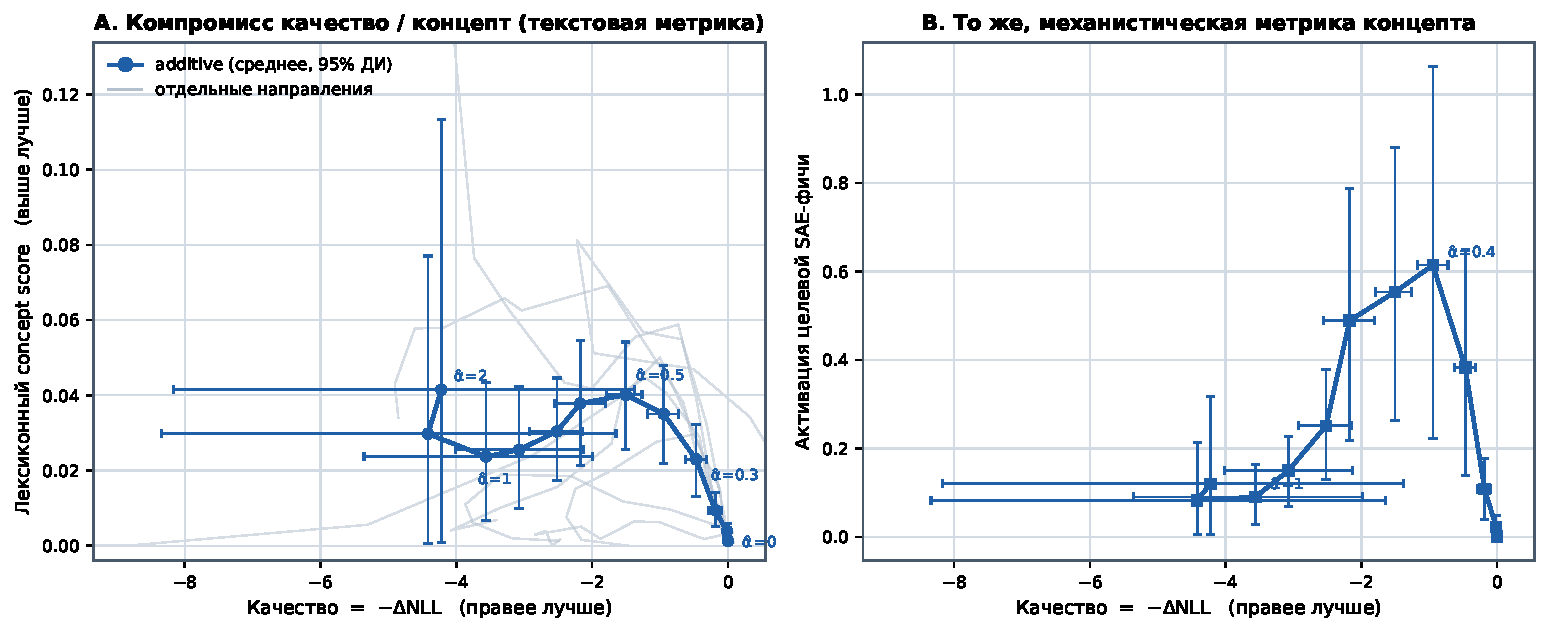
\includegraphics[width=\textwidth]{figures/fig01_additive_pareto.pdf}
  \caption{Обычный аддитивный стиринг создаёт компромисс качество\,$\leftrightarrow$\,концепт.
  Слева — текстовая метрика, справа — механистическая. Тонкие линии — отдельные
  направления; бутстрэп по направлениям, не по генерациям. 8 DEV-направлений
  $\times$ 30 промптов на конфигурацию.}
  \label{fig:additive}
\end{figure}

\begin{center}\small
\begin{tabular}{@{}rrrrrr@{}}
\toprule
$\ahat$ & $\Delta$NLL & лексикон & SAE-фича & Dist-2 & повторы\\
\midrule
0    & $+0.0000$ & 0.0012 & 0.0018 & 0.9858 & 0.0019\\
0.3  & $+0.4693$ & 0.0230 & 0.3828 & 0.9881 & 0.0025\\
\textbf{0.4} & $+0.9463$ & 0.0350 & \textbf{0.6145} & 0.9886 & 0.0038\\
\textbf{0.5} & $+1.5037$ & \textbf{0.0401} & 0.5539 & 0.9859 & 0.0076\\
0.7  & $+2.5192$ & 0.0304 & 0.2516 & 0.9705 & 0.0313\\
1.0  & $+3.5614$ & 0.0237 & 0.0909 & 0.8349 & 0.0526\\
2.0  & $+4.2220$ & 0.0415 & 0.1206 & 0.6608 & 0.0808\\
\bottomrule
\end{tabular}
\end{center}

\medskip
Три наблюдения определяют весь дальнейший анализ.

\begin{enumerate}
  \item \textbf{Концепт немонотонен.} Активация целевой SAE-фичи достигает
    максимума при $\ahat = 0.4$ и затем обрушивается: при $\ahat = 1.0$ она в
    6.8 раза ниже пика: дальнейшее увеличение $\ahat$ не усиливает SAE-сигнал и
резко ухудшает качество.
  \item \textbf{Полезная рабочая зона узкая}: $\ahat \approx 0.3$--$0.5$. Именно
    в ней осмысленно спрашивать про улучшение.
  \item \textbf{Рост лексикона при $\ahat = 2.0$ обманчив.} Он сопровождается
    Dist-2 $= 0.66$ и долей повторов $0.081$: это лексическое затопление
    вырожденным текстом \cite{holtzman2020degeneration}, а не выражение
    концепта. Лексиконную метрику нельзя читать в отрыве от диагностик деградации.
\end{enumerate}

%==============================================================================
\section{Дешёвый гауссов денойзер из задания}

Остаточный MLP над активациями остаточного потока, обученный по классической
схеме обучения денойзера \cite{vincent2008denoising}:
\[
  \mathcal{L} = \lVert h - D(h + \varepsilon)\rVert^2,
  \qquad \varepsilon \sim \mathcal{N}(0, \sigma^2 I).
\]
При применении к стирингу денойзер действует непосредственно на активацию после стиринга:
$\tilde h = D(h + \alpha v)$.

\textbf{Что именно было обучено.} Остаточный MLP над сырыми активациями
остаточного потока в той же точке \texttt{blocks.7.hook\_resid\_pre};
повреждение — масштабированный гауссов шум, \textbf{без использования информации
о направлениях стиринга}. Функциональная реконструкция измерялась при
$\sigma \in \{0.25, 0.5, 1.0, 2.0\}$ относительно масштаба активаций
$\mathbb{E}\lVert h\rVert = 88.76$.

Веса и конфигурация обучения этого раннего варианта не сохранились, поэтому
архитектурные детали (ширины слоёв, оптимизатор, объём обучающих активаций) мы не
приводим, чтобы не выдать правдоподобную реконструкцию за факт. Четыре значения
реконструкции ниже взяты из зафиксированной экспериментальной записи; поведение
денойзера \emph{на стиринге} пересчитано полностью.

\subsection{Вспомогательная задача решена}

\begin{figure}[H]
  \centering
  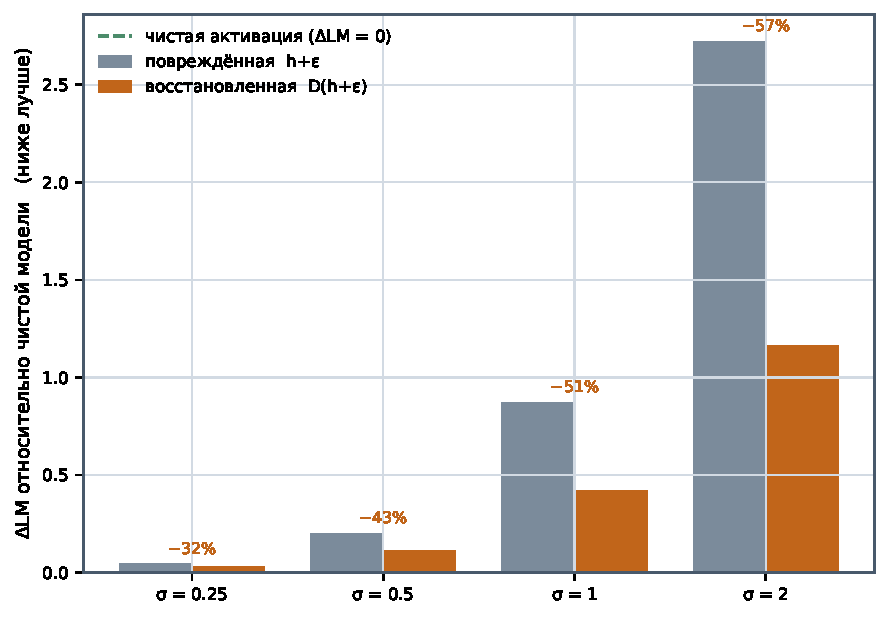
\includegraphics[width=0.80\textwidth]{figures/fig04_denoiser_ability.pdf}
  \caption{Денойзер из задания действительно решает свою задачу: гауссово
  повреждение естественных активаций восстанавливается на 32--57\,\%.}
  \label{fig:denoiser}
\end{figure}

\begin{center}\small
\begin{tabular}{@{}rrrr@{}}
\toprule
$\sigma$ & $\Delta$LM повреждённой & $\Delta$LM восстановленной & восстановлено\\
\midrule
0.25 & 0.0451 & 0.0307 & 32\,\%\\
0.50 & 0.1997 & 0.1138 & 43\,\%\\
1.00 & 0.8722 & 0.4239 & 51\,\%\\
2.00 & 2.7236 & 1.1619 & 57\,\%\\
\bottomrule
\end{tabular}
\end{center}

\medskip
\textbf{Сеть является настоящим функциональным денойзером.} Дальнейший
отрицательный результат нельзя объяснить тем, что «денойзер плохо обучился».

\subsection{На стиринге устойчивого выигрыша нет}

\begin{figure}[H]
  \centering
  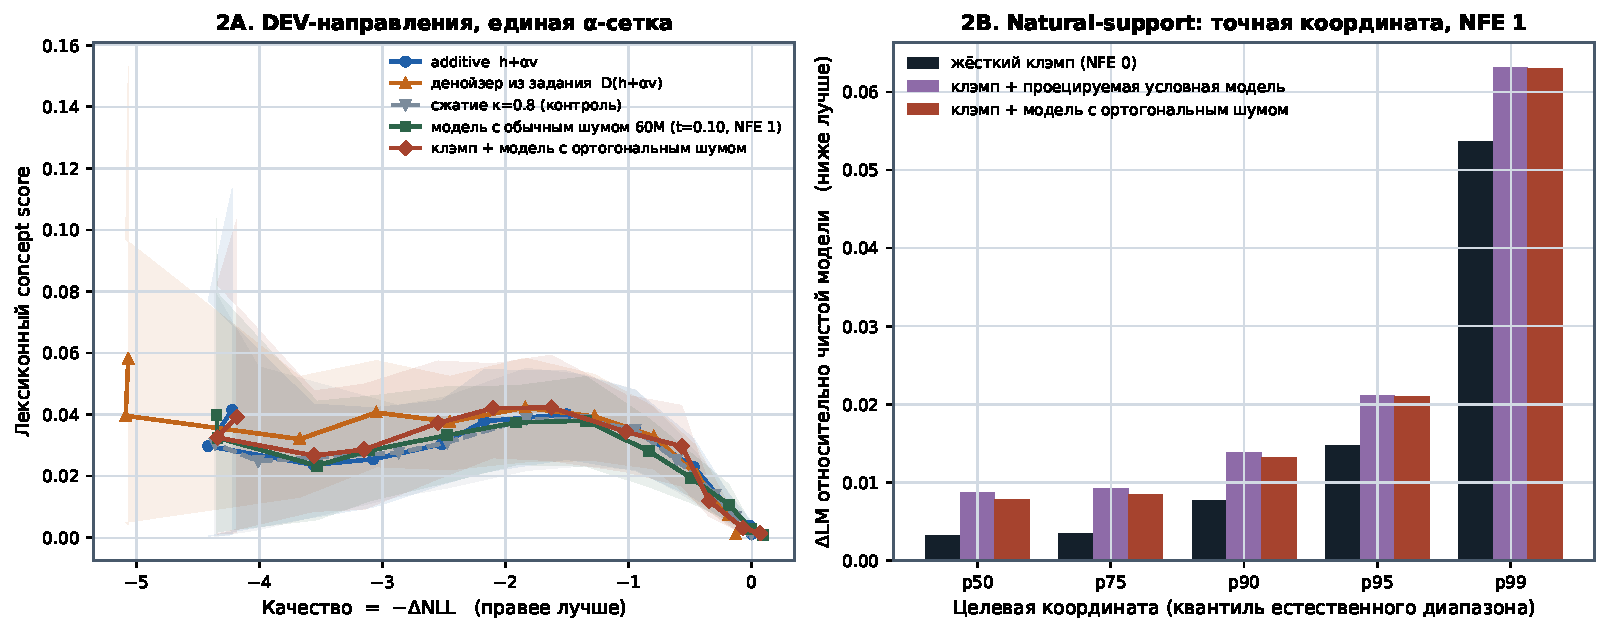
\includegraphics[width=\textwidth]{figures/fig02_method_comparison.pdf}
  \caption{Сравнение методов. Слева — общая $\ahat$-сетка на DEV-направлениях,
  справа — точная координата из естественного диапазона. Панели \emph{не}
  объединены: у них разные определения осей — слева концепт задаётся $\alpha$,
  справа абсолютной координатой.}
  \label{fig:comparison}
\end{figure}

В панели A все пять методов ложатся практически на одну кривую. При равной
номинальной $\alpha$ денойзер иногда выигрывает по NLL — но, как показано ниже,
это не улучшение активации.

%==============================================================================
\section{Номинальный выигрыш объясняется ослаблением стиринга}\label{sec:attenuation}

Коррекция денойзера $c = D(h + \alpha v) - z$ раскладывается на компоненты вдоль
$v$ и ортогонально ему. Измеренная геометрия:

\begin{center}\small
\begin{tabular}{@{}rrrrr@{}}
\toprule
$\ahat$ & $\cos(c, v)$ & $\lVert c_{\parallel}\rVert$ & $\lVert c_{\perp}\rVert$ & стирания стиринга\\
\midrule
0.3 & $-0.475$ & 4.99 & 8.33 & 18.8\,\%\\
0.5 & $-0.548$ & 8.71 & 12.07 & 19.6\,\%\\
1.0 & $-0.585$ & 21.71 & 28.66 & 24.5\,\%\\
2.0 & $-0.596$ & 48.71 & 63.75 & 27.4\,\%\\
\bottomrule
\end{tabular}
\end{center}

\medskip
Косинус устойчиво отрицателен: \textbf{коррекция систематически направлена
против стиринга}.

Это качественно ожидаемо. Для \emph{оптимального} MSE-денойзера при гауссовом
шуме поправка $D(z) - z$ связана с градиентом логарифма зашумлённой плотности активаций
$p_\sigma$ формулой Tweedie \cite{efron2011tweedie}:
$\mathbb{E}[h \mid z] = z + \sigma^2 \nabla_z \log p_\sigma(z)$. Активация после стиринга $z = h + \alpha v$ лежит в области меньшей плотности, поэтому
компонента коррекции, направленная обратно к областям большей вероятностной
массы, — то есть против $v$, — ожидаема.

Это мотивация и интерпретация, а не доказательство для конкретной сети:
обученный денойзер конечной ёмкости не равен идеальному оценщику градиента логарифма плотности, и
измеренный косинус ($-0.475\ldots-0.596$) не является проверкой этого
тождества. Наблюдаемая картина такова:
\[
  D(h + \alpha v) \;\approx\; h + \alpha_{\mathrm{eff}} v
  \;+\; (\text{вредная ортогональная коррекция}),
  \qquad \alpha_{\mathrm{eff}} < \alpha .
\]
Улучшение NLL при меньшем $\alpha_{\mathrm{eff}}$ — это движение по уже
известной кривой аддитивного стиринга, а не новый фронт.

\begin{figure}[H]
  \centering
  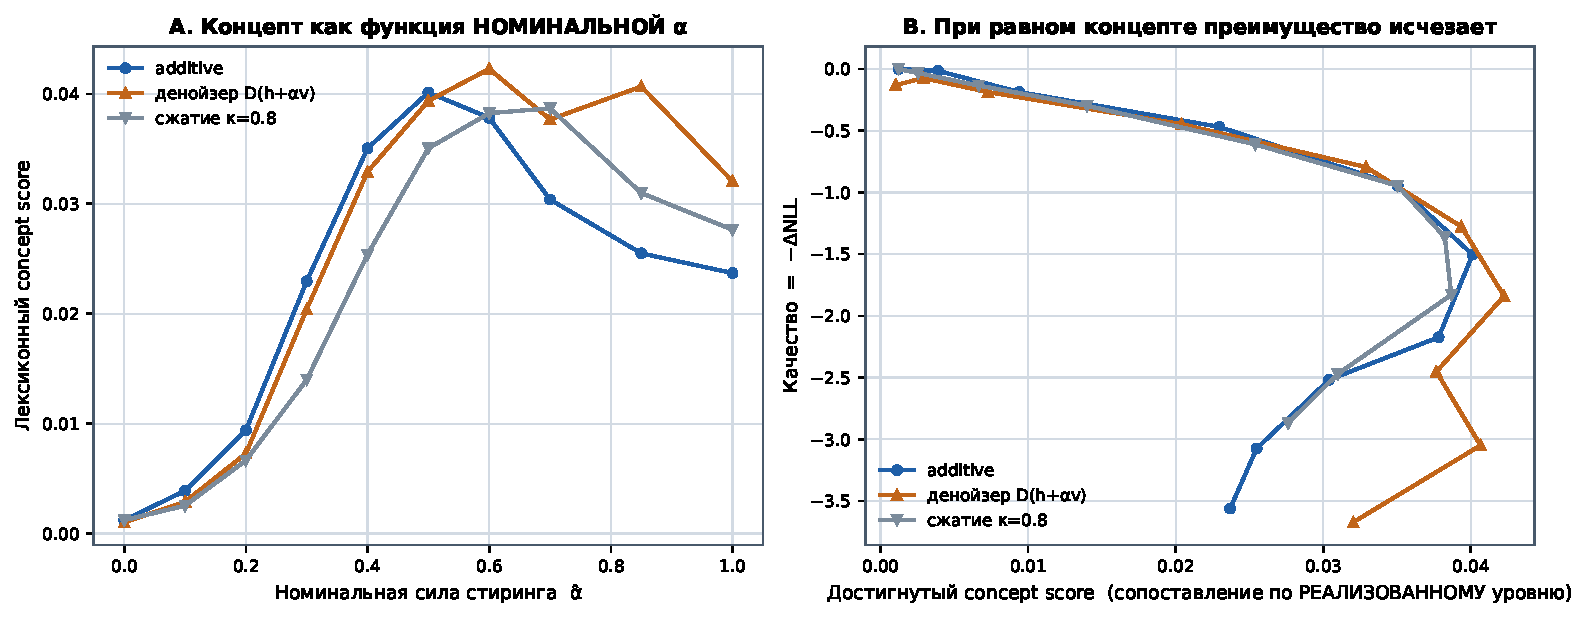
\includegraphics[width=\textwidth]{figures/fig03_matched_strength.pdf}
  \caption{Ослабление стиринга против настоящей коррекции. Если кривая
  метода в панели B совпадает с кривой аддитивного стиринга, его выигрыш по NLL объясняется
  меньшим эффективным $\alpha$, а не улучшением активации. Основная
  $\ahat$-сетка, без стресс-точек.}
  \label{fig:matched}
\end{figure}

Панель B — решающая проверка. При отложенном \emph{фактически достигнутом}
уровне концепта кривые денойзера и сжатия $\kappa = 0.8$ ложатся на кривую
аддитивного стиринга в рабочей зоне. Преимущество исчезает.

Дополнительные диагностические проверки согласуются с этим выводом:
коррекция только вдоль направления $v$ работала заметно лучше полной; фиксированное сжатие
$\kappa \approx 0.8$ воспроизводило большую часть эффекта; а вариант без параллельной компоненты
(убрать компоненту вдоль $v$, оставить только ортогональную) качество
\emph{ухудшал}. Последнее — первое прямое указание, что ортогональная коррекция
денойзера вредна; к этому мы вернёмся в \S\ref{sec:mechanism}.

%==============================================================================
\section{Более мощная генеративная модель}\label{sec:capacity}

Гипотеза: денойзер слишком прост, и для восстановления активаций нужна
более выразительная генеративная модель. В Generative Latent Prior
\cite{luo2026glp} для этого обучают модель распределения естественных активаций и
используют её для коррекции после стиринга. Наш вариант намеренно дешёвый:
flow matching
\cite{lipman2023flowmatching,liu2023rectifiedflow} в стандартизованном
пространстве активаций (линейный путь, $t=0$ — данные, $t=1$ — шум, цель
$u^{*} = \varepsilon - x_0$); при применении используется схема SDEdit
\cite{meng2022sdedit} с малым числом вычислений сети.

Мы \emph{не} воспроизводим GLP буквально: там существенно больший масштаб
модели и данных. Интересующий нас режим — маленькая модель, активации
GPT-2-масштаба, дешёвое обучение и очень мало вызовов сети при применении.

\begin{figure}[H]
  \centering
  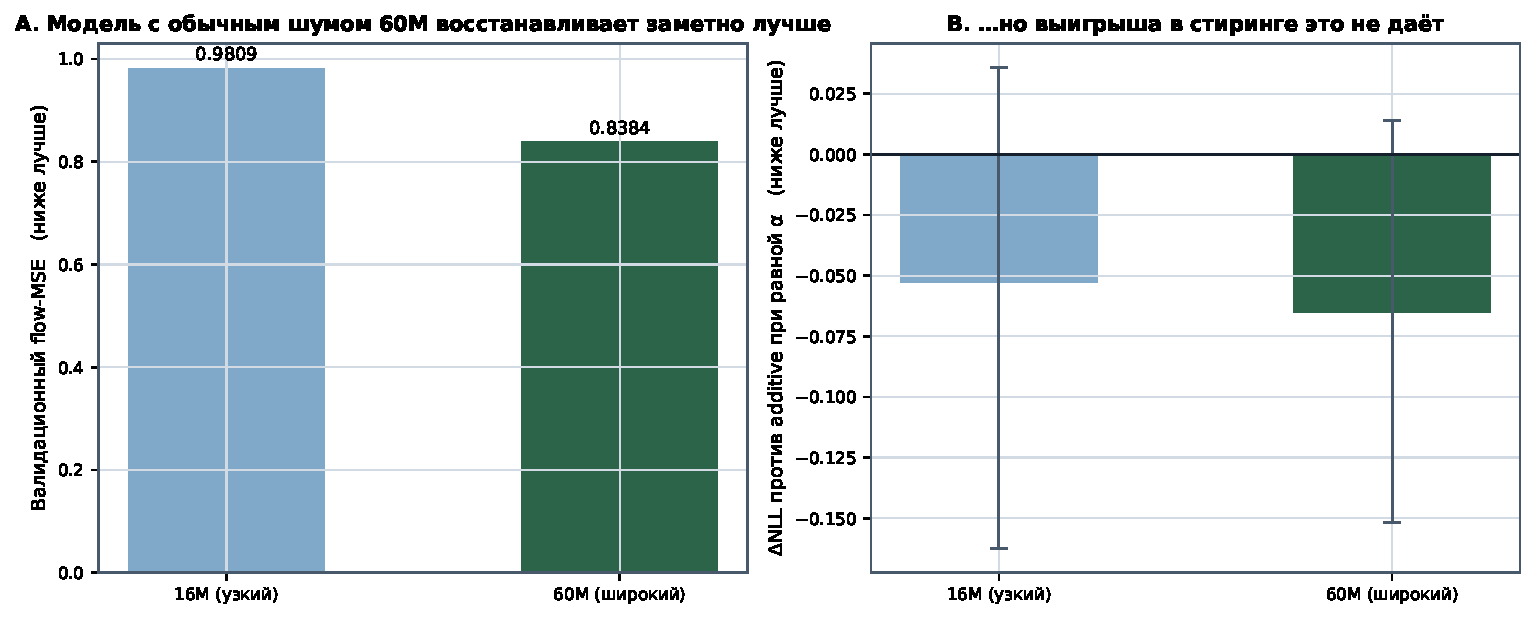
\includegraphics[width=\textwidth]{figures/fig05_capacity_transfer.pdf}
  \caption{Лучшая реконструкция активаций $\not\Rightarrow$ лучшая коррекция
  стиринга. Увеличение размера модели с 16M до 60M улучшает flow-MSE на
  14.5\,\%, но не даёт статистически различимого выигрыша в стиринге.}
  \label{fig:capacity}
\end{figure}

\begin{center}\small
\begin{tabular}{@{}lrr@{}}
\toprule
 & 16M (узкий) & 60M (широкий)\\
\midrule
Валидационный flow-MSE & 0.9809 & \textbf{0.8384}\\
$\Delta$NLL относительно аддитивного стиринга при равной $\alpha$ & $-0.0530\;[-0.1626, +0.0358]$ & $-0.0654\;[-0.1518, +0.0142]$\\
\bottomrule
\end{tabular}
\end{center}

\medskip
Модель на 60M существенно лучше восстанавливает активации (flow-MSE ниже на
14.5\,\%). Но выигрыш на стиринге у обеих статистически неотличим от нуля:
доверительные интервалы пересекают ноль, а изменения концепта тем более
(лексикон $-0.0008\,[-0.0029, +0.0009]$).

\textbf{Неудачу модели с обычным шумом нельзя объяснить только недостаточной
ёмкостью 16M-модели:} увеличение ёмкости до 60M заметно улучшило метрику
реконструкции, но не дало статистически различимого выигрыша в стиринге. Это
утверждение относится только к этому варианту; вопрос ёмкости модели с
ортогональным шумом остаётся открытым (\S\ref{sec:limits}).

%==============================================================================
\section{Условные модели и точное сохранение линейной координаты}

\subsection{Модель, знающая желаемую координату}

Следующее объяснение: модель не знает, какую именно координату надо
сохранить. Обучена условная модель $f(x_t, t, v, c)$, где $c = \langle h, v\rangle$.
Здесь и далее речь идёт о \textbf{выбранной линейной координате стиринга}
$\langle h, v\rangle$, а не о семантике концепта как таковой: диагностика
\S\ref{sec:curvature} показывает, что условные средние естественных активаций нелинейно зависят от этой координаты.

\begin{figure}[H]
  \centering
  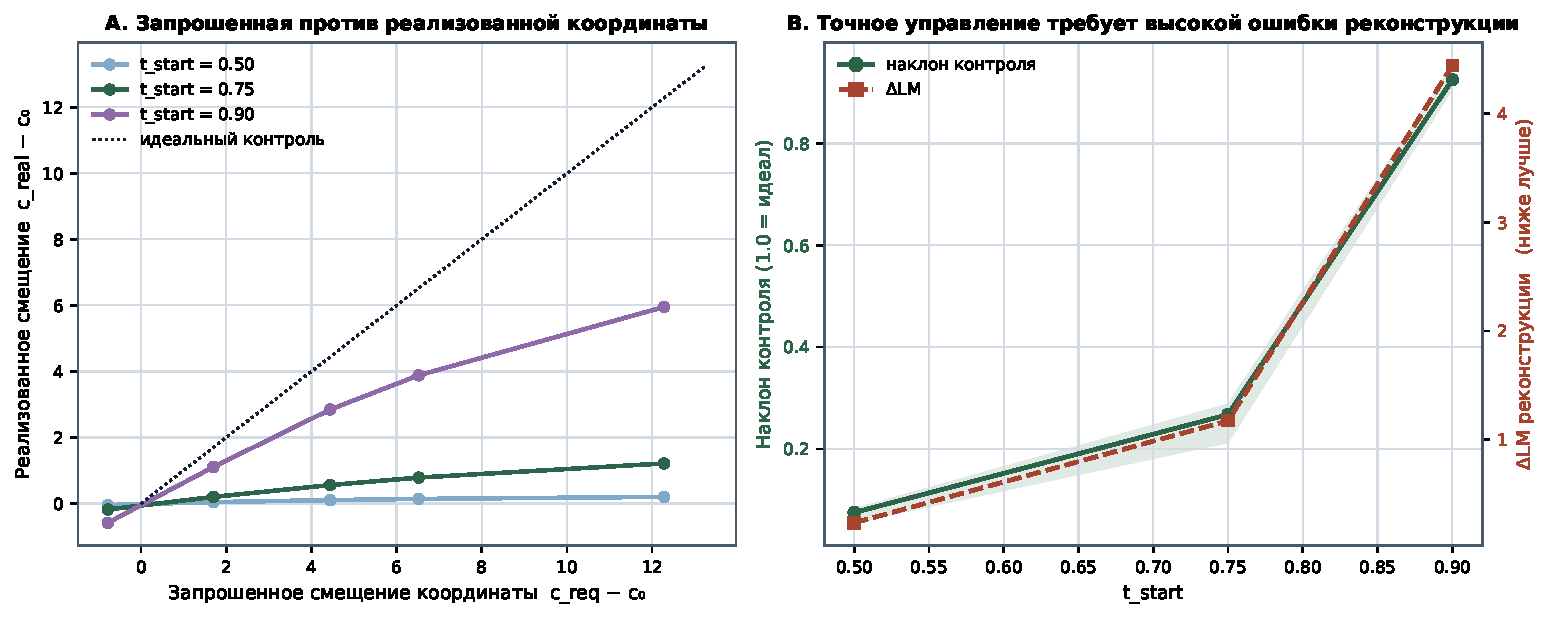
\includegraphics[width=\textwidth]{figures/fig06_conditional_control.pdf}
  \caption{Условная модель управляет координатой, но цена растёт быстрее.
  Панель B — среднее по пяти целевым квантилям, полоса — разброс между ними.
  Сильное управление появляется только там, где одна лишь реконструкция уже
  стоит дорого.}
  \label{fig:conditional}
\end{figure}

\begin{center}\small
\begin{tabular}{@{}rrcr@{}}
\toprule
$t_{\mathrm{start}}$ & наклон контроля & разброс по квантилям & $\Delta$LM (цена)\\
\midrule
0.50 & 0.075 & 0.055--0.083 & 0.234\\
0.75 & 0.268 & 0.212--0.288 & 1.174\\
0.90 & \textbf{0.925} & 0.906--0.953 & \textbf{4.444}\\
\bottomrule
\end{tabular}
\end{center}

\medskip
Условное управление \textbf{работает}: при $t_{\mathrm{start}} = 0.90$ наклон 0.925
близок к идеальной единице и однороден по квантилям. Но точное управление
достигается ценой резкого роста ошибки реконструкции: в той же точке одна лишь
реконструкция стоит $\approx 4.44$ ната, что операционно неприемлемо.

\subsection{Жёсткий клэмп: сильный бейзлайн}

Это мотивирует простой аналитический бейзлайн — жёсткий клэмп.
\[
  h_{\mathrm{clamp}} = h + (c_{\mathrm{target}} - \langle h, v\rangle)\, v .
\]

\begin{figure}[H]
  \centering
  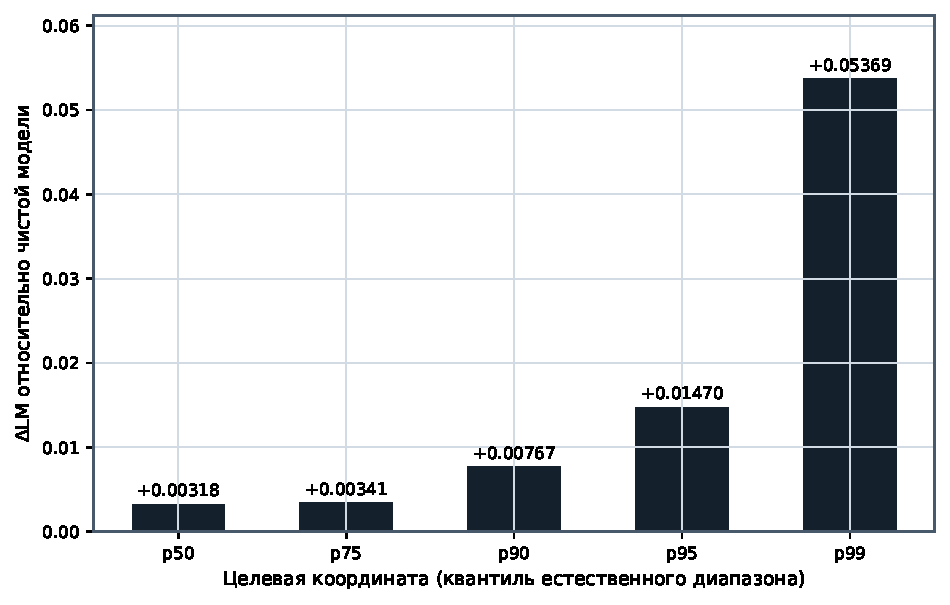
\includegraphics[width=0.66\textwidth]{figures/fig07_hard_clamp_cost.pdf}
  \caption{Точный жёсткий клэмп стоит очень дёшево: от $+0.003$ до $+0.054$ ната
  при ошибке координаты порядка $10^{-6}$. Это тот бейзлайн, который не смог
  превзойти ни один генеративный метод.}
  \label{fig:clamp}
\end{figure}

Это тот бейзлайн, который в дальнейшем не смог превзойти ни один генеративный
метод. Заодно клэмп закрывает лазейку: раз координата задана точно, метод больше
не может «выиграть» за счёт её ослабления.

%==============================================================================
\section{Потоковая модель с ортогональным шумом}

Последнее оставшееся объяснение — различие между шумом при обучении и тем,
что требуется от модели при применении. Предыдущие потоковые модели обучались с
обычным гауссовым шумом, который меняет активацию во всех направлениях, а после
клэмпа от них требовалось исправлять только компоненты, ортогональные направлению
стиринга, не меняя заданную координату.

Поэтому в последнем варианте шум при обучении сразу ограничен ортогональным
подпространством: из него удаляется компонента вдоль $v$. Для чистой
стандартизованной активации $x_0$, единичного направления $v$ и координаты
$c = \langle x_0, v\rangle$:
\begin{align}
  x_{\parallel} &= c\,v, &
  x_{\perp} &= x_0 - c\,v, &
  \varepsilon_{\perp} &= \varepsilon - \langle \varepsilon, v\rangle v,\\
  x_t &= c\,v + (1-t)\,x_{\perp} + t\,\varepsilon_{\perp}
    &&\Longrightarrow\; \langle x_t, v\rangle = c \;\;\forall t, \notag\\
  u^{*} &= \varepsilon_{\perp} - x_{\perp}
    &&\Longrightarrow\; \langle u^{*}, v\rangle = 0. \notag
\end{align}

Используемая скорость аналитически проецируется:
$u - \langle u, v\rangle v$. Ограничение — свойство метода, а не то, чему сеть
учится. Это важно для чтения результата: отрицательный итог нельзя объяснить
уходом координаты.

Модель: 16\,542\,464 параметра, 250\,000 шагов, FineWeb-32M, только
обучающий пул направлений. Отбор чекпоинта — по валидационному flow-MSE, без
участия каких-либо метрик стиринга.

\subsection{T1 — модель решает свою задачу}

\begin{figure}[H]
  \centering
  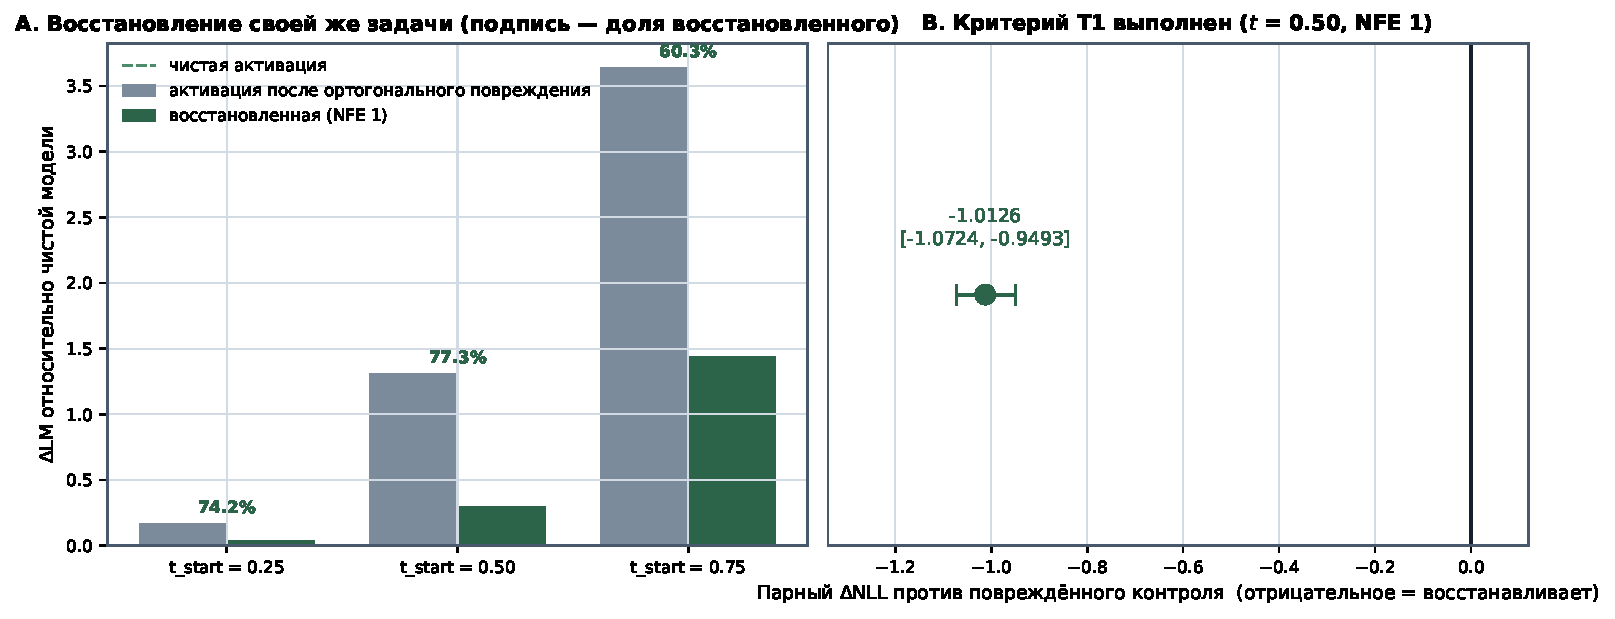
\includegraphics[width=\textwidth]{figures/fig08_t1_reconstruction.pdf}
  \caption{T1 — модель с ортогональным шумом уверенно решает свою задачу. Порог доли
  восстановленного 0.25 задан до получения данных; фактически 0.7730.
  Бутстрэп кластеризован по направлениям.}
  \label{fig:t1}
\end{figure}

\begin{center}\small
\begin{tabular}{@{}rrrr@{}}
\toprule
$t_{\mathrm{start}}$ & $\Delta$LM повреждённой & $\Delta$LM восстановленной & восстановлено\\
\midrule
0.25 & 0.16701 & 0.04305 & 74.2\,\%\\
\textbf{0.50} & 1.30996 & 0.29735 & \textbf{77.3\,\%}\\
0.75 & 3.64025 & 1.44405 & 60.3\,\%\\
\bottomrule
\end{tabular}
\end{center}

\medskip
В основной заранее выбранной конфигурации ($t_{\mathrm{start}} = 0.50$, NFE 1)
критерий T1 выполнен. Парный
$\Delta$NLL против повреждённого контроля $-1.012611$, 95\,\% ДИ
$[-1.072443, -0.949261]$. Валидационный MSE на задаче с ортогональным шумом равен 0.9662
против 1.9951 у нулевого предсказателя.

\subsection{T2 — коррекция после клэмпа всё равно не помогает}

\begin{figure}[H]
  \centering
  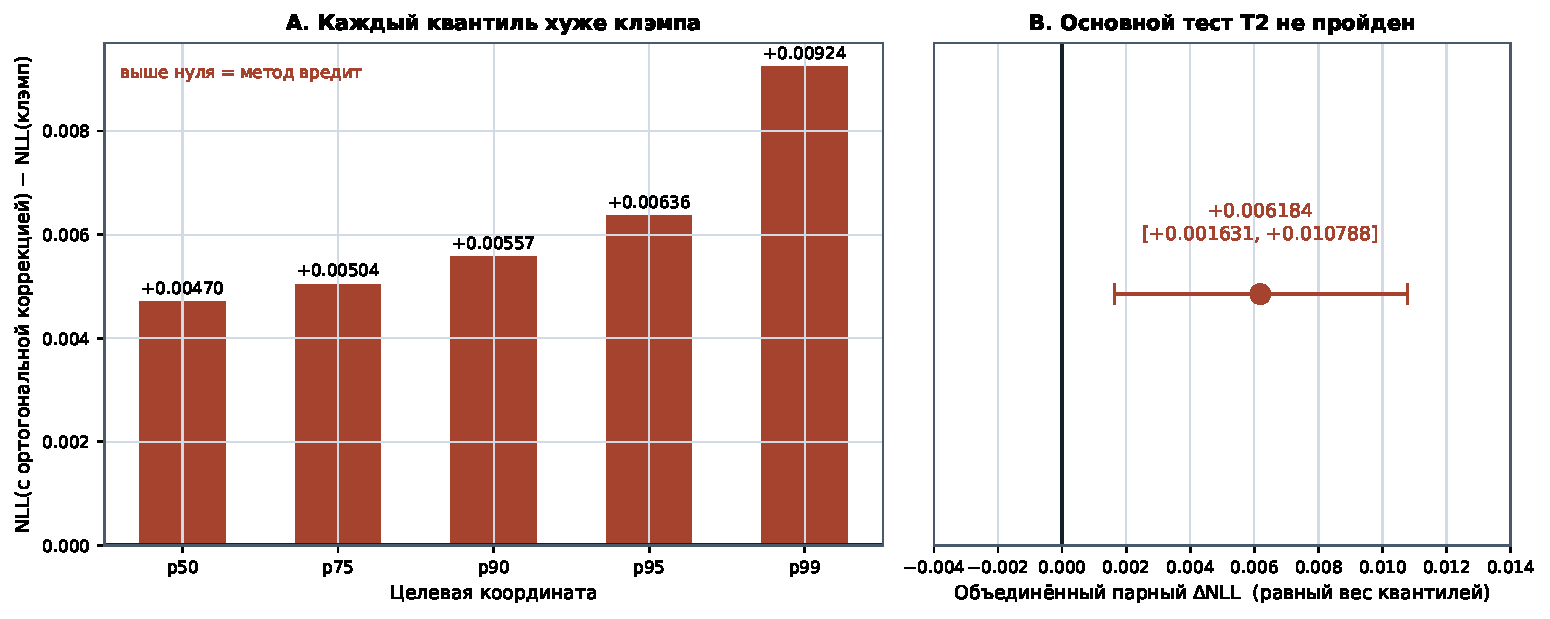
\includegraphics[width=\textwidth]{figures/fig09_t2_naturalization.pdf}
  \caption{T2 — коррекция после клэмпа не помогает при точно фиксированной координате.
  ни одна из 30 дополнительных конфигураций не дала улучшения; направлений с отрицательным
  эффектом 25\,\% при пороге $>$80\,\%. LOVO $[+0.005244, +0.006816]$ —
  ноль не пересекается.}
  \label{fig:t2}
\end{figure}

Два варианта при \textbf{одинаковой} точно зафиксированной координате: жёсткий клэмп
и клэмп + потоковая модель с ортогональным шумом. Заранее выбранная рабочая точка
$t_{\mathrm{start}} = 0.10$, NFE 1, объединение по пяти квантилям с равным весом.

\begin{center}\small
\begin{tabular}{@{}lrrr@{}}
\toprule
Целевая координата & NLL клэмпа & NLL с коррекцией & $\Delta$NLL\\
\midrule
p50 & 3.77339 & 3.77809 & $+0.004702$\\
p75 & 3.77362 & 3.77866 & $+0.005042$\\
p90 & 3.77788 & 3.78345 & $+0.005572$\\
p95 & 3.78490 & 3.79127 & $+0.006363$\\
p99 & 3.82389 & 3.83313 & $+0.009241$\\
\bottomrule
\end{tabular}
\end{center}

\medskip
\textbf{Объединённый $\Delta\mathrm{NLL} = +0.006184$, 95\,\% ДИ
$[+0.001631, +0.010788]$.}

Знак положительный, интервал не пересекает ноль. Робастность не выполнена ни по
одному критерию: отрицательный эффект лишь у 8 из 32 направлений (25\,\%, нужно
$>80\,\%$), LOVO-диапазон $[+0.005244, +0.006816]$ нуля не пересекает.
\textbf{Ни одна из 30 дополнительных конфигураций не дала улучшения.}

%==============================================================================
\section{Почему метод не сработал}\label{sec:mechanism}

Первое подозрение при таком результате — ослабление координаты. Здесь оно
исключено конструктивно и подтверждено измерениями:

\begin{center}\small
\begin{tabular}{@{}lr@{}}
\toprule
Величина & Значение\\
\midrule
средняя параллельная коррекция $\dhpar$ & $5.61\times10^{-7}$\\
средняя ортогональная коррекция $\dhperp$ & $7.085$\\
отношение $\dhpar / \dhperp$ & $7.9\times10^{-8}$\\
максимальная ошибка координаты & $5.72\times10^{-6}$\\
максимальное расхождение между вариантами & $9.54\times10^{-6}$\\
допуск критерия совпадения координат & $1.0\times10^{-3}$\\
\bottomrule
\end{tabular}
\end{center}

\medskip
Максимальное расхождение между вариантами $< 10^{-5}$ при допуске $10^{-3}$, то есть
на два порядка внутри требования. Модель двигала \textbf{только} ортогональные
степени свободы — и заметно (относительная $L_2$ к чистой активации 0.113).

\subsection{Ущерб растёт вместе с нормой ортогональной коррекции}

\begin{center}\small
\begin{tabular}{@{}rrr@{}}
\toprule
$t_{\mathrm{start}}$ & $\dhperp$ & объединённый $\Delta$NLL\\
\midrule
0.10 & 7.09 & $+0.006184$\\
0.25 & 16.81 & $+0.054130$\\
0.50 & 29.58 & $+0.346458$\\
\bottomrule
\end{tabular}
\end{center}

\begin{figure}[H]
  \centering
  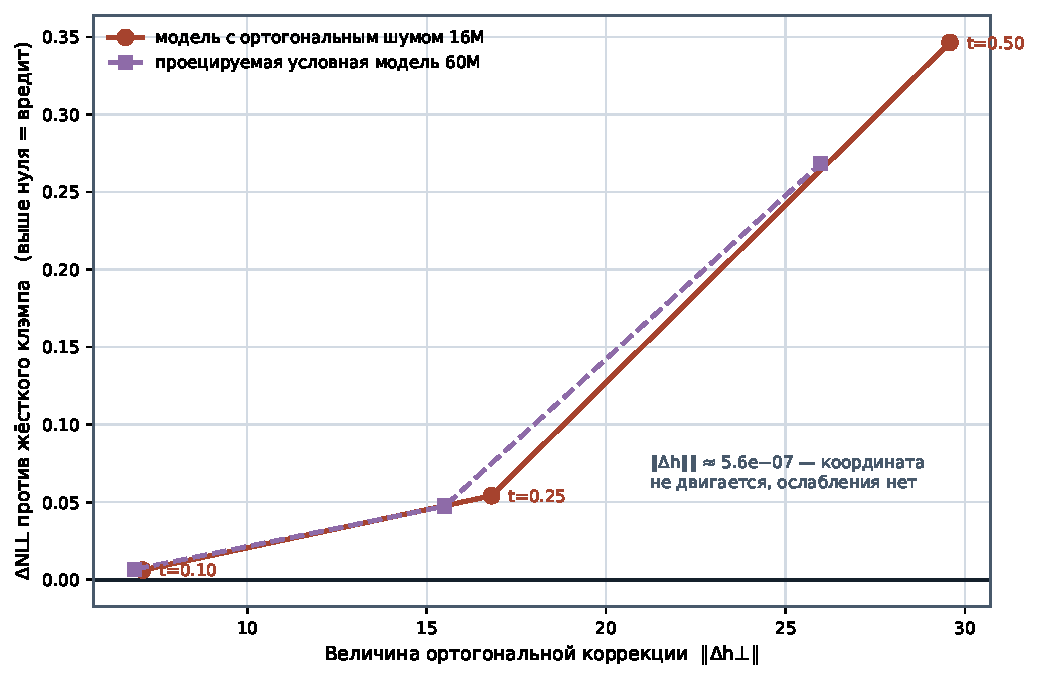
\includegraphics[width=0.78\textwidth]{figures/fig10_mechanism.pdf}
  \caption{Ущерб растёт вместе с величиной ортогональной коррекции: обе кривые
  монотонны и почти совпадают.
  \textbf{Сопоставление диагностическое, не причинное:} модели различаются по
  ёмкости (61.0M против 16.5M), поэтому близость кривых \emph{не} позволяет
  изолировать эффект выбора целевой функции обучения.}
  \label{fig:mechanism}
\end{figure}

Зависимость монотонная и ускоряющаяся. Формулировка, ровно соответствующая
данным:

\begin{quote}
В обеих проверенных схемах и на трёх значениях $t_{\mathrm{start}}$ ущерб
монотонно растёт вместе с нормой ортогональной коррекции.
\end{quote}

Сопоставление с ранее проверенной моделью с обычным шумом на том же плане
($t_{\mathrm{start}} = 0.10$, NFE 1):

\begin{center}\small
\begin{tabular}{@{}lrr@{}}
\toprule
Целевая координата & модель с обычным шумом 60M (с проекцией) & модель с ортогональным шумом 16M\\
\midrule
p50 & $+0.005493$\;($\dhperp$ 6.75) & $+0.004702$\;(7.02)\\
p75 & $+0.005790$\;(6.76) & $+0.005042$\;(7.03)\\
p90 & $+0.006119$\;(6.82) & $+0.005572$\;(7.06)\\
p95 & $+0.006488$\;(6.88) & $+0.006363$\;(7.09)\\
p99 & $+0.009429$\;(7.11) & $+0.009241$\;(7.23)\\
\bottomrule
\end{tabular}
\end{center}

\medskip
Переход от обычного шума к ортогональному снизил $\Delta$NLL лишь на несколько
тысячных ната и не изменил знак эффекта. Модели различаются по ёмкости в 3.7 раза, поэтому это \emph{наблюдение}, а
не изоляция вклада целевой функции; согласованный контроль по ёмкости не проводился
(\S\ref{sec:limits}).

\textbf{Проверка валидности.} Результат для жёсткого клэмпа воспроизвёлся между двумя
запусками точно ($+0.00318 / +0.00341 / +0.00767 / +0.01470 / +0.05369$ на
p50\ldots p99 в обоих).

%==============================================================================
\section{Финальный метод на задаче из ТЗ}\label{sec:dev}

Оценки T1/T2 подменяют активации и не порождают текст, поэтому у модели с
ортогональным шумом не было ни Dist-$n$, ни точки на DEV-Парето. Пробел закрыт отдельным
прогоном по \textbf{тому же DEV-протоколу}: те же промпты, $\ahat$-сетка,
seeds, декодирование и метрики, что у остальных методов; 2880 парных сравнений.

Вмешательство: клэмп к координате, эквивалентной аддитивному стирингу
$c = \langle h, v\rangle + \alpha$, затем коррекция потоковой моделью с ортогональным шумом при точно
удержанной координате. Существенная деталь: \textbf{сам клэмп на этой сетке в
точности совпадает с аддитивным вмешательством $h+\alpha v$}, поэтому отдельным вариантом он не идёт — измеряется только
вклад потоковой модели. Оценка выполнена после основного эксперимента и
носит описательный характер: заранее зафиксированного критерия успеха для неё не
было, и результат T2 она не меняет.

\begin{figure}[H]
  \centering
  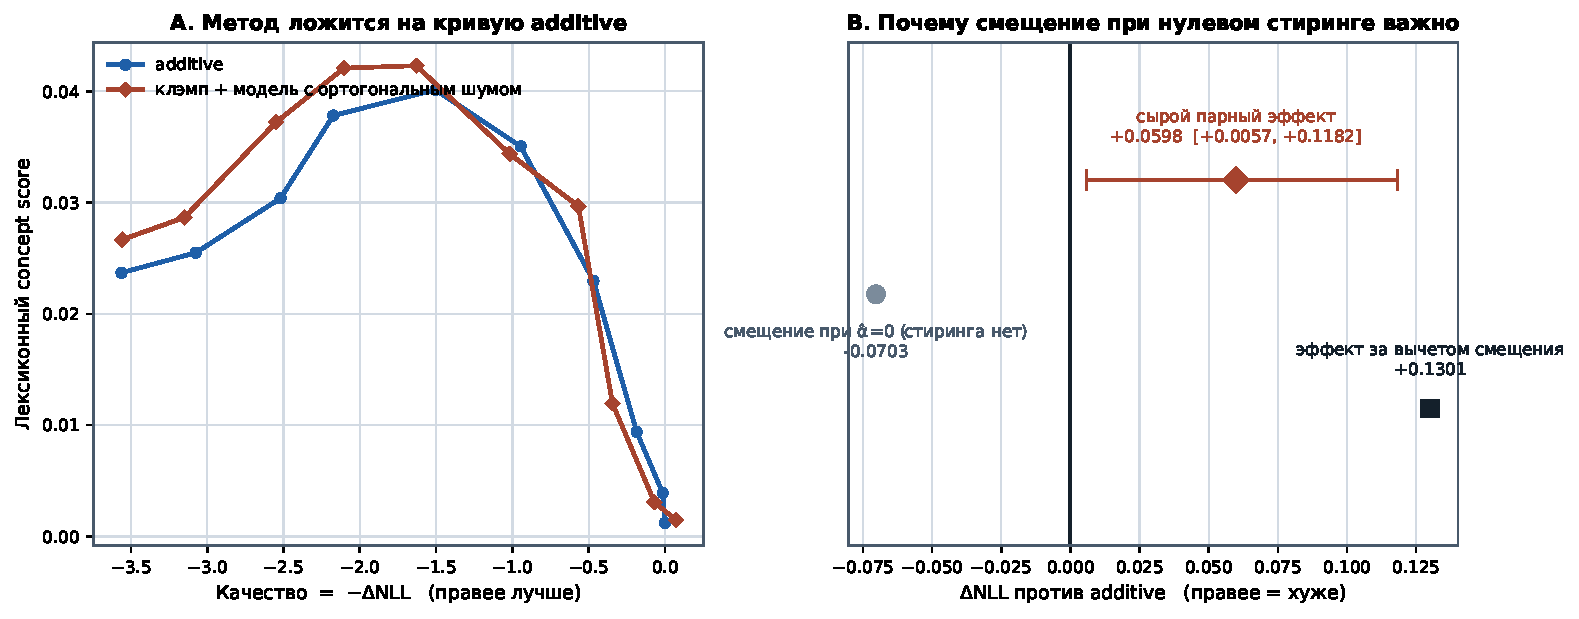
\includegraphics[width=\textwidth]{figures/fig11_tangent_on_dev.pdf}
  \caption{Финальный метод на задаче из ТЗ (дополнительная оценка вне основного
  протокола). Кривая метода практически совпадает с кривой аддитивного стиринга; 2880 парных сравнений,
  бутстрэп по направлениям. При $\ahat=0$ клэмп тождествен, поэтому $-0.070$
  ната — изменение чистой активации, а не выигрыш стиринга.}
  \label{fig:dev}
\end{figure}

\subsection{Контроль при нулевом стиринге и поправка на смещение}

При $\ahat = 0$ целевая координата равна собственной координате активации, клэмп
становится тождеством, и потоковая модель меняет уже \emph{чистую} активацию. Там метод
\textbf{снижает} условную NLL на 0.070 ната. Это сдвиг базовой линии, а не
выигрыш в стиринге, поэтому специфичный для стиринга эффект определяется как
разность разностей:
\begin{equation}
  \Delta_{\text{steering-specific}}
  = \bigl[\mathrm{NLL}_F(\alpha) - \mathrm{NLL}_A(\alpha)\bigr]
  - \bigl[\mathrm{NLL}_F(0) - \mathrm{NLL}_A(0)\bigr],
  \label{eq:did}
\end{equation}
где $F$ — модель с ортогональным шумом, $A$ — аддитивный стиринг.

\begin{center}\small
\begin{tabular}{@{}lr@{}}
\toprule
Величина & Значение\\
\midrule
сырой парный $\Delta$NLL относительно аддитивного стиринга ($\ahat \in 0.1\ldots1.0$) & $\mathbf{+0.0598}$\\
95\,\% ДИ (бутстрэп по направлениям) & $[+0.0057, +0.1182]$\\
направлений с улучшением & 2 из 8\\
смещение при $\ahat = 0$ (стиринга нет) & $\mathbf{-0.0703}$\\
$\Delta_{\text{steering-specific}}$ по \eqref{eq:did} & $\mathbf{+0.1301}$\\
\bottomrule
\end{tabular}
\end{center}

\medskip
Сырой парный эффект уже включает это базовое смещение; по \eqref{eq:did} вред метода при
ненулевом стиринге составляет $+0.1301$ ната — в 2.2 раза больше. Приведены обе
величины; ни одна не подгонялась.

Вывод согласуется с T2, но получен на другой постановке — на DEV-векторах с
текстовой метрикой концепта, то есть прямо на языке исходного задания.

%==============================================================================
\section{Dist-1/2/3 и диагностики генерации}

\begin{center}\small
\begin{tabular}{@{}lrrrrrr@{}}
\toprule
Метод & $\ahat$ & NLL & Dist-1 & Dist-2 & Dist-3 & повторы\\
\midrule
чистая модель & — & 3.4393 & 0.8508 & 0.9858 & 0.9983 & 0.0019\\
аддитивный & 0.3 & 3.9086 & 0.8574 & 0.9881 & 0.9969 & 0.0025\\
аддитивный & 0.6 & 5.6130 & 0.8501 & 0.9809 & 0.9969 & 0.0158\\
аддитивный & 1.0 & 7.0007 & 0.7762 & 0.8349 & 0.8311 & 0.0526\\
денойзер $D(h{+}\alpha v)$ & 0.3 & 3.8866 & 0.8641 & 0.9904 & 0.9987 & 0.0006\\
денойзер $D(h{+}\alpha v)$ & 0.6 & 5.2792 & 0.8453 & 0.9824 & 0.9964 & 0.0099\\
денойзер $D(h{+}\alpha v)$ & 1.0 & 7.1117 & 0.7869 & 0.8723 & 0.8841 & 0.0532\\
сжатие $\kappa{=}0.8$ & 0.6 & 4.8007 & 0.8654 & 0.9887 & 0.9979 & 0.0060\\
потоковая модель 60M (обычный шум) & 0.6 & 5.3512 & 0.8382 & 0.9797 & 0.9964 & 0.0175\\
клэмп + модель с ортогональным шумом & 0.3 & 4.0074 & 0.8683 & 0.9899 & 0.9978 & 0.0018\\
клэмп + модель с ортогональным шумом & 0.6 & 5.5424 & 0.8381 & 0.9798 & 0.9949 & 0.0202\\
клэмп + модель с ортогональным шумом & 1.0 & 6.9962 & 0.7793 & 0.8398 & 0.8297 & 0.0523\\
\bottomrule
\end{tabular}
\end{center}

\medskip
До $\ahat \approx 0.6$ разнообразие практически не страдает, а при $\ahat = 1.0$
обрушивается у всех методов. По разнообразию модель с ортогональным шумом неотличима от
аддитивного стиринга. \textbf{Dist-$n$ здесь — дешёвая диагностика уровня генерации, а не
полноценная метрика беглости}; первичной метрикой качества остаётся условная NLL.

Жёсткий клэмп отдельной строки не требует: на координате, эквивалентной аддитивному стирингу,
он тождественно совпадает с аддитивным вмешательством. Для клэмпа с \emph{абсолютными} координатами
естественного диапазона Dist-$n$ не считался — это другое семейство оценок, где
концепт задаётся не через $\alpha$.

%==============================================================================
\section{Дополнительные проверки}\label{sec:poststop}

Проверки A--D выполнены после основного результата T1/T2 и рассматриваются как
дополнительные анализы, уточняющие возможные объяснения отрицательного
результата, а не как его пересмотр.

\subsection{A — путь с сохранением дисперсии}\label{sec:vp}

Возможное объяснение отрицательного результата: линейный путь повреждения
$x_t = (1-t)x_0 + t\epsilon$ схлопывает масштаб активации по мере роста $t$, и
модель могла учиться работать с неестественно сжатыми состояниями. Проверка —
путь с сохранением дисперсии, сравниваемый с линейным
при \textbf{согласованной тяжести} повреждения
$t_{\mathrm{vp}} = \tfrac{2}{\pi}\arctan\!\big(t_{\mathrm{lin}}/(1-t_{\mathrm{lin}})\big)$,
а не при равном $t$.

\begin{figure}[H]
  \centering
  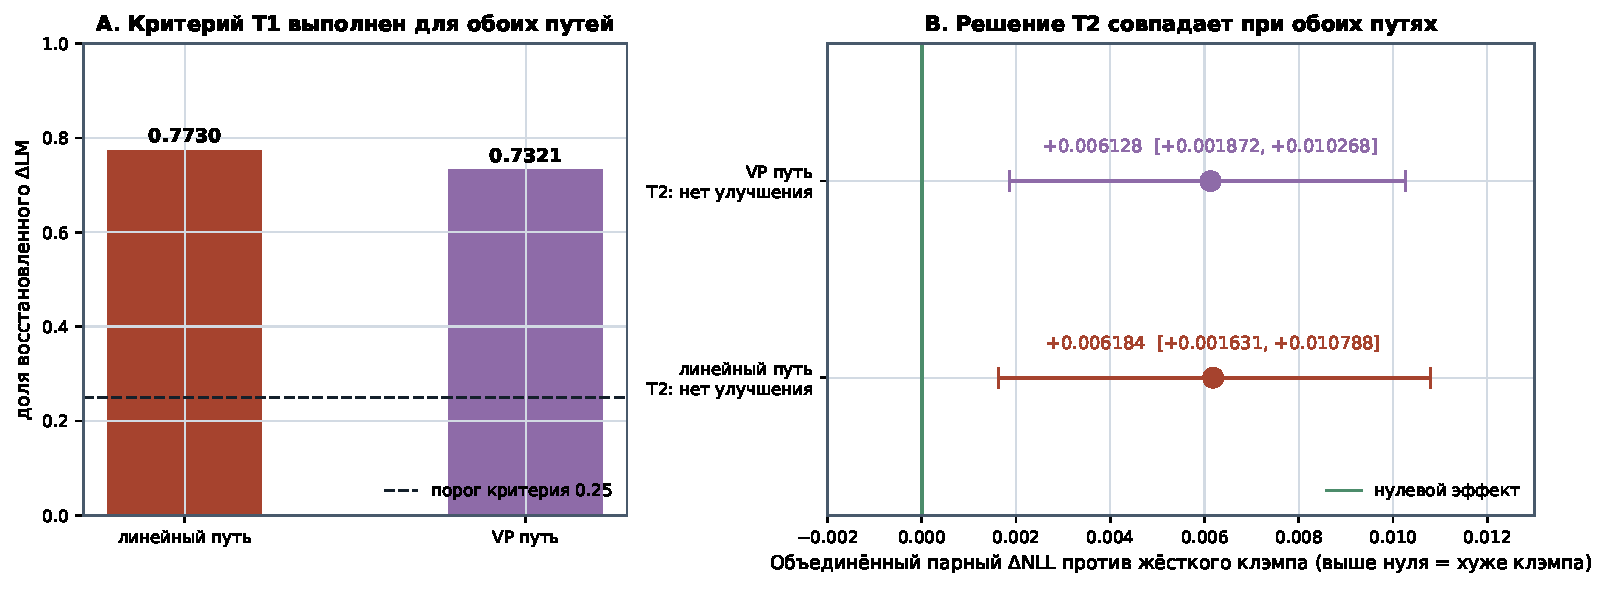
\includegraphics[width=\textwidth]{figures/fig12_vp_path_control.pdf}
  \caption{Смена геометрии пути не меняет результата. Оба пути выполняют
  критерий T1 и оба не проходят T2 практически с одинаковым числом.}
  \label{fig:vp}
\end{figure}

\begin{center}\small
\begin{tabular}{@{}lrrl@{}}
\toprule
Путь & T1 (доля восстановленного) & T2 (объединённый $\Delta$NLL) & 95\,\% ДИ\\
\midrule
линейный & 0.7730 & $+0.006184$ & $[+0.001631, +0.010788]$\\
с сохранением дисперсии & 0.7321 & $+0.006128$ & $[+0.001872, +0.010268]$\\
\bottomrule
\end{tabular}
\end{center}

\medskip
Критерий T1 выполнен на обоих путях, тест T2 не пройден ни на одном; ни одна
из 30 дополнительных конфигураций не дала улучшения. Контроль целостности
сравнения: жёсткий клэмп пересчитывается внутри того же прогона и воспроизвёл
опубликованные значения $+0.003184 / +0.003414 / +0.007674 / +0.014700 / +0.053689$
\textbf{в точности}, поэтому оба числа T2 сопоставимы.

\textbf{Вывод A:} схлопывание масштаба вдоль линейного пути не объясняет
отрицательный результат — путь с сохранением дисперсии воспроизводит его
практически без изменений. Это \emph{не} закрывает вопрос о любом несоответствии
процессов повреждения: несоответствие «гауссово против стиринг-подобного»
проверяется отдельно (\S\ref{sec:denoiserB}).

Сырой валидационный flow-MSE $= 1.47663$ нельзя сравнивать напрямую с
flow-MSE линейного пути: целевая скорость на VP-пути имеет другой масштаб
из-за множителя $\pi/2$. Отбор чекпоинта проводился внутри одного прогона по
своей же метрике и остаётся концепт-независимым.

\subsection{B — денойзер стиринг-подобного повреждения}\label{sec:denoiserB}

Последнее прямое объяснение отрицательного результата — несоответствие процесса
повреждения. Все предыдущие модели обучались на гауссовом (или ортогональном)
шуме, а исправлять от них требовалось совсем другое искажение: смещение вдоль
$v$. Поэтому обучен денойзер прямо на нём:
\[
  z = h + \delta v, \qquad D(z) \to h, \qquad
  \delta \sim \mathcal{U}[-32, 32],
\]
с направлениями только из обучающего пула. Диапазон $\delta$ зафиксирован до
любой оценки, из опубликованных смещений жёсткого клэмпа. Отбор чекпоинта — по
своей же реконструкционной метрике, валидационный flow-MSE $= 0.0288773$, без
единой метрики стиринга.

При применении проверялась частичная коррекция
$h'_\lambda = z + \lambda\,(D(z) - z)$ на заранее фиксированной сетке
$\lambda \in \{0.25, 0.5, 0.75, 1.0\}$; решающая точка — $\lambda = 1.00$.

\begin{figure}[H]
  \centering
  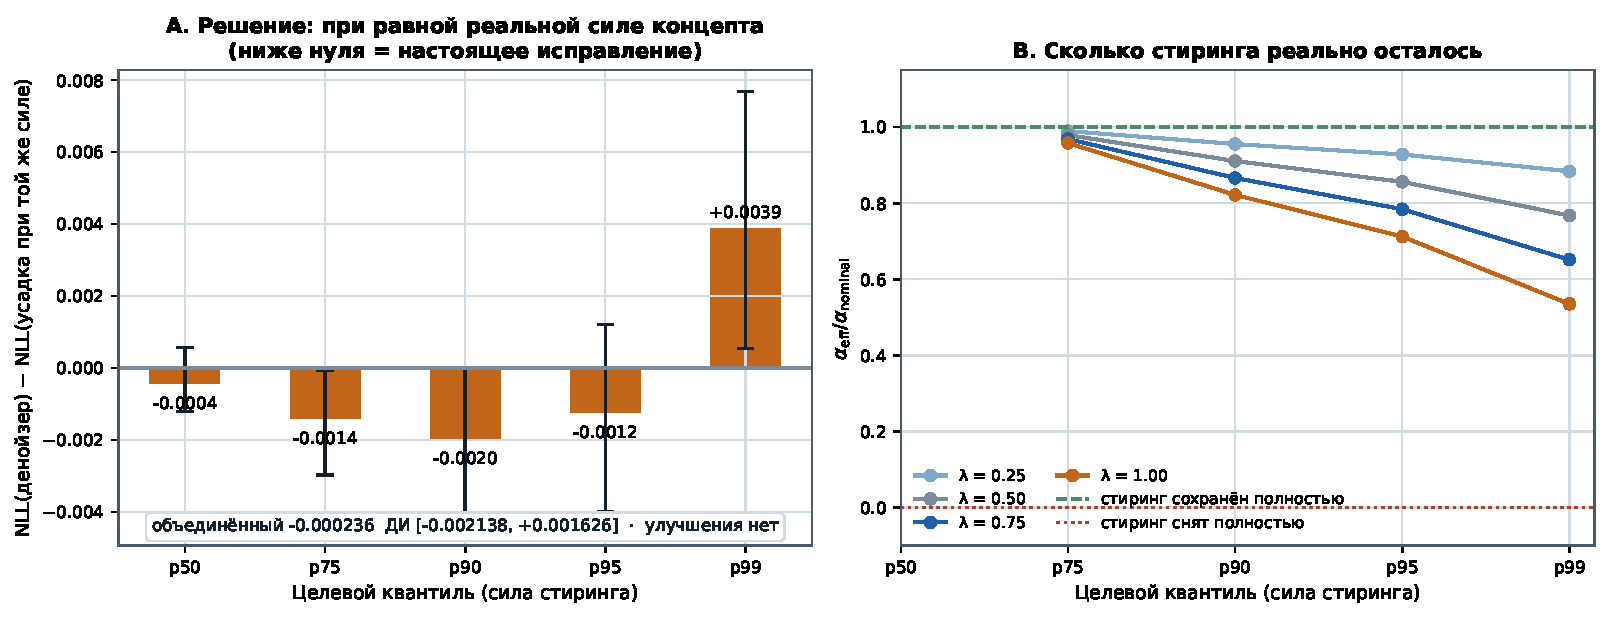
\includegraphics[width=\textwidth]{figures/fig13_steering_denoiser_matched.pdf}
  \caption{Денойзер, обученный прямо на стиринг-подобном повреждении. Панель A —
  сравнение при равной \emph{реально достигнутой} силе концепта; панель B —
  сколько стиринга при этом осталось.}
  \label{fig:denoiserB}
\end{figure}

\textbf{При номинальном сравнении метод выглядит успешным.} Против аддитивного
стиринга при той же номинальной $\alpha$ денойзер выигрывает на каждой ступени,
и выигрыш растёт с $\lambda$: $-0.00044$ / $-0.00156$ / $-0.00456$ / $-0.00934$ /
$-0.04032$ ната при p50\ldots p99.

\textbf{Но стиринга к этому моменту почти не остаётся.} Доля сохранённой силы
$\alpha_{\mathrm{eff}}/\alpha_{\mathrm{nominal}}$ при $\lambda = 1.00$:

\begin{center}\small
\begin{tabular}{@{}lrrrr@{}}
\toprule
$\lambda$ & p75 & p90 & p95 & p99\\
\midrule
0.25 & 0.9895 & 0.9554 & 0.9280 & 0.8838\\
0.50 & 0.9790 & 0.9109 & 0.8561 & 0.7676\\
0.75 & 0.9685 & 0.8663 & 0.7841 & 0.6514\\
1.00 & 0.9580 & 0.8218 & 0.7122 & \textbf{0.5352}\\
\bottomrule
\end{tabular}
\end{center}

\medskip
На самой сильной ступени денойзер снимает почти половину стиринга. Зависимость
монотонна по обеим осям: чем больше коррекция, тем меньше остаётся концепта и
тем «лучше» выглядит номинальное сравнение.

\textbf{Решение принимается при равной реальной силе.} Контроль — скалярная
усадка, которой построчно задана ровно та же $\alpha_{\mathrm{eff}}$, что
получилась у денойзера. Совпадение силы проверено: максимальное расхождение
между плечами $3.8\times10^{-6}$ при допуске $10^{-3}$, то есть на два с
половиной порядка внутри требования на всех пяти ступенях.

\begin{center}\small
\begin{tabular}{@{}lr@{}}
\toprule
Величина & Значение\\
\midrule
объединённый парный $\Delta$NLL & $-0.000236$\\
95\,\% ДИ & $[-0.002138, +0.001626]$\\
направлений с отрицательным эффектом & 15 из 32 (46.9\,\%)\\
LOVO-диапазон & $[-0.000581, +0.000390]$\\
\bottomrule
\end{tabular}
\end{center}

\medskip
Интервал накрывает ноль, направления делятся почти пополам, LOVO нуля не
избегает. \textbf{Улучшения нет.}

\textbf{Вывод B:} обучение на стиринг-подобном повреждении в основном научило
модель \emph{отменять} стиринг, а не естественным образом исправлять
активацию после стиринга. Весь номинальный выигрыш объясняется ослаблением: при
равной реально достигнутой силе концепта преимущества над простой усадкой нет.
Тем самым закрывается и последнее прямое объяснение через несоответствие
процессов повреждения.

Побочное наблюдение: на ступени $\alpha = 0$ денойзер тоже слегка улучшает NLL
($-0.00044$), то есть часть номинального выигрыша вообще не связана со стирингом
и представляет собой шумоподавление чистой активации.

\subsection{C — нелинейная геометрия условных средних}\label{sec:curvature}

Все предыдущие методы использовали $\langle h, v\rangle$ как выбранную линейную
координату силы вмешательства. Диагностика C проверяет, насколько естественные
активации меняются линейно при движении вдоль этой координаты: активации
разбиваются по
квантилям собственной координаты, берутся секанты между средними соседних
корзин $d_k = \mu_{k+1} - \mu_k$, и измеряется, поворачиваются ли они с ростом
выбранной линейной координаты. Аффинное условное среднее дало бы
$\cos(d_k, d_{k+1}) = 1$ точно. Диагностика ничего не обучает и не применяет
языковую модель.

\textbf{Первоначальный результат.} Недобор до потолка надёжности $0.2805$,
ДИ $[0.2461, 0.3110]$, 32/32 направлений положительны, LOVO $[0.2760, 0.2868]$.
Потолок split-half $0.9950$: шумом оценки средних по корзинам это не
объясняется. Перемешивание соответствия «активация~$\to$~корзина» разрушает
структуру полностью — $\cos(d_k, d_{k+1})$ падает с $0.7145$ до $-0.4624$, парная
разница $+1.1768$, ДИ $[+1.1424, +1.2140]$. Тот же пайплайн на 32
непересекающихся направлениях, которые использовали эксперименты со стирингом,
воспроизводит недобор $0.2544$, ДИ $[0.2159, 0.2960]$.

\subsubsection*{Почему выравнивание с $v$ нельзя читать напрямую}

Напрашивающееся сравнение — $\cos(d_k, v)$ против случайных единичных осей —
неинформативно: эта величина сильно зависит от того, сколько дисперсии несёт
направление, а случайная единичная ось в 768 измерениях несёт её очень мало
(\S\ref{sec:refusalD}).

У этого есть точная причина. Для гауссовой популяции
\[
  E[h \mid v^\top h = c]
  = \mu + \frac{\Sigma v}{v^\top \Sigma v}\,(c - v^\top\mu),
\]
то есть линейное направление условной траектории задаётся не самим $v$, а
$\Sigma v$. Остаточный поток сильно анизотропен, поэтому уход условного среднего
«в сторону от $v$» — это \emph{ожидаемое} поведение чисто линейной гауссовой
популяции, а не признак изгиба. Измерено прямо: $\cos(d_k, v) = 0.375$, тогда как
$\cos(d_k, \Sigma v) = \mathbf{0.745}$. Траектория следует ковариационному
предсказанию вдвое точнее, чем самому $v$.

\begin{quote}
$\cos(d_k, v)$ здесь приводится как описательная статистика. Она смешана с
ковариацией активаций и \textbf{не} интерпретируется как свидетельство о
касательности или о причинных свойствах направления.
\end{quote}

\subsubsection*{Ковариационные контроли (C6)}

Проверка, какая часть результата переживает контроль на геометрию ковариации.
Ничего не обучается; критерии зафиксированы до вычислений.

\begin{figure}[H]
  \centering
  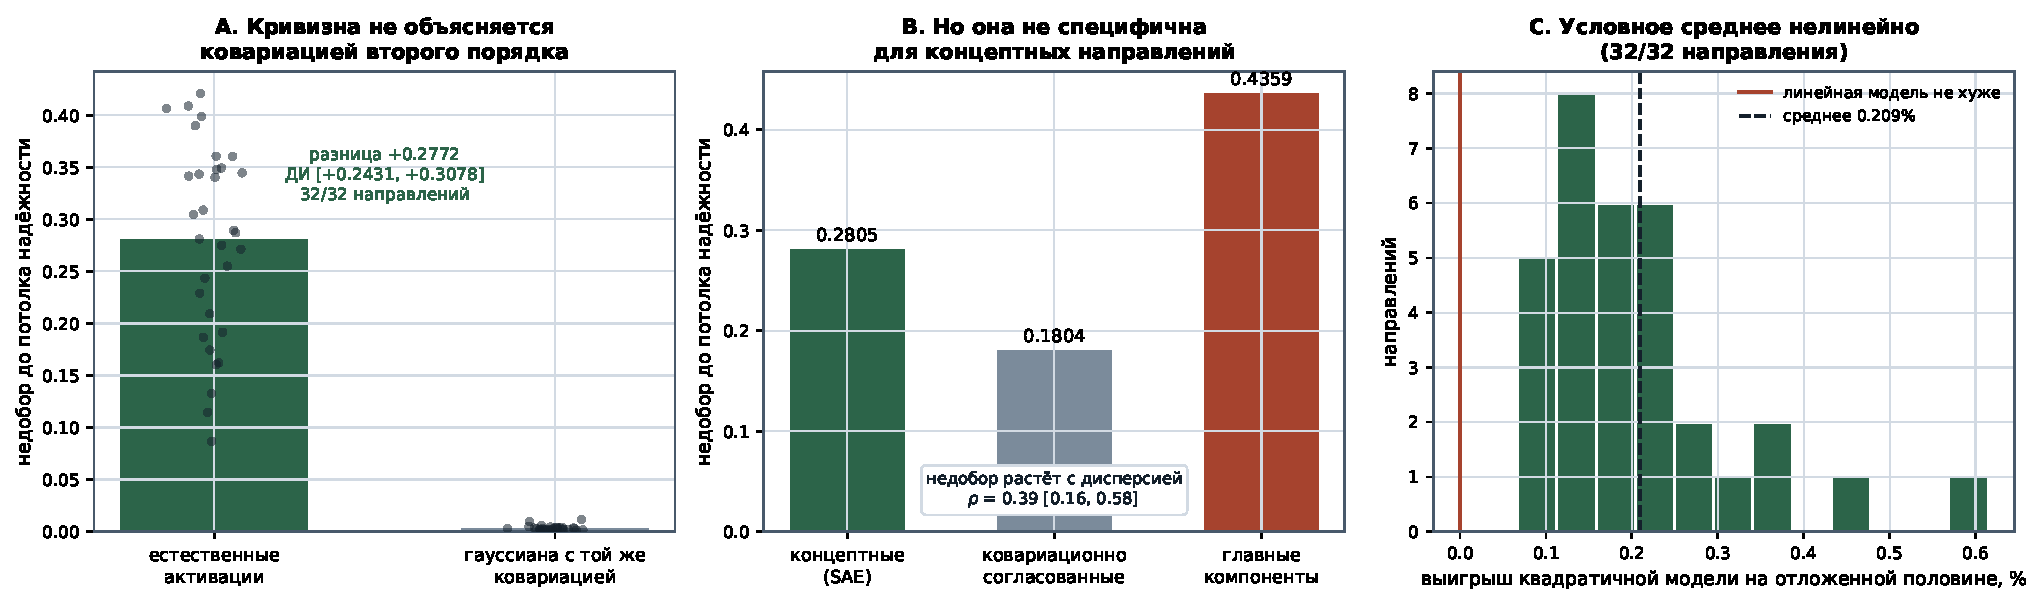
\includegraphics[width=\textwidth]{figures/fig14_concept_curvature.pdf}
  \caption{Кривизна после ковариационных контролей. Панель A — сравнение с
  гауссовой популяцией, у которой \emph{та же} ковариация. Панель B — концептные
  направления против ковариационно согласованных случайных и против главных
  компонент. Панель C — выигрыш квадратичной условной модели на отложенной
  половине.}
  \label{fig:curvature}
\end{figure}

\textbf{Что выживает.} Два контроля согласованы по дисперсии по построению, и оба
дают однозначный ответ.

\emph{Гауссовый суррогат.} Сгенерирована популяция $\mathcal N(\hat\mu,
\hat\Sigma)$ с той же эмпирической ковариацией (относительная ошибка
воспроизведения $0.026$), тем же числом строк и размерностью. Её условное среднее
линейно по построению, поэтому любая кривизна на ней — артефакт конечной выборки
и самого пайплайна. Недобор на суррогате $\mathbf{0.0033}$ против
$\mathbf{0.2805}$ на настоящих активациях; разница $+0.2772$, ДИ
$[+0.2431, +0.3078]$, 32/32 направлений. Сравнение парное: то же $v$, та же
проецируемая дисперсия.

\emph{Отложенная квадратичная модель.} Последовательности разбиты пополам;
на одной половине подгоняется $h \approx a + b_1 c$ и $h \approx a + b_1 c +
b_2 c^2$, качество измеряется на другой. Квадратичная модель выигрывает на
\textbf{32 направлениях из 32}: $\Delta$MSE $= +0.0116$, ДИ
$[+0.0096, +0.0140]$, относительный выигрыш $0.209\,\%$, ДИ
$[0.173\,\%, 0.253\,\%]$. Остаточные условные средние после вычитания линейной
модели составляют $0.52$ от локальной секанты, то есть систематическая структура
сохраняется. Эта проверка вообще не использует углы и потому не может быть
смешана с анизотропией.

\textbf{Что не выживает.} Утверждение, что концептные направления искривлены
\emph{сильнее прочих}, контроля не проходит.

Согласовать случайные оси по ковариации не удалось: из 20000 кандидатов
ближайшие по паре $(\log v^\top\Sigma v,\ \cos(v,\Sigma v))$ всё равно несут
вдвое меньшую проецируемую дисперсию (8.06 против 17.09), а по второй переменной
баланс даже ухудшился. Причина структурная: случайные единичные направления в
768 измерениях концентрируются в узком диапазоне дисперсии ($4.8$–$7.1$), тогда
как концептные достигают $59.0$. Подходящих кандидатов в пуле просто нет.

Это важно, потому что недобор \textbf{растёт} с проецируемой дисперсией:
$\rho = 0.39$, ДИ $[0.16, 0.58]$ по 72 направлениям. Поэтому превышение над
согласованным нуллом ($+0.1001$, ДИ $[+0.0642, +0.1367]$) нельзя отнести на счёт
концептности. Решает прямое сравнение: главные компоненты,
отобранные \emph{только} по дисперсии и не имеющие никакого концептного смысла,
искривлены \textbf{сильнее} концептных направлений — недобор $0.4359$ против
$0.2805$.

\textbf{Итоговая формулировка C:}

\begin{quote}
Условные средние естественных активаций меняются вдоль выбранной линейной
координаты стиринга \textbf{нелинейно}, и этот эффект не объясняется ни шумом
оценки, ни ковариационной геометрией второго порядка. Но он \textbf{не специфичен
для концептных направлений}: направления, отобранные по одной лишь дисперсии,
искривлены сильнее.
\end{quote}

Растущий профиль $\cos(d_k, v)$ (0.294, 0.346, 0.359, 0.375, 0.503; контраст
«хвост минус центр» $+0.1444$, ДИ $[+0.1068, +0.1796]$) воспроизводится и на
заведомо причинном направлении в другой модели (\S\ref{sec:refusalD}), поэтому
сам по себе он ничего не говорит об управляемости и в отчёте так не
используется.

\subsection{D — положительный контроль на заведомо причинном направлении}\label{sec:refusalD}

Результат C допускал два несовместимых прочтения. Либо SAE-направление — плохая
ось вмешательства, и отсутствие выравнивания объясняет провал коррекции. Либо
выравнивание с касательной естественной траектории вообще не является свойством,
которое нужно причинному направлению, — и тогда C ничего не говорит о
управляемости. Различить их можно только одним способом: прогнать ту же
диагностику на направлении, про которое независимо известно, что вмешательство
вдоль него меняет поведение.

Взято опубликованное refusal-направление из работы Arditi и соавт.
\cite{arditi2024refusal} для \texttt{google/gemma-2b-it}: слой 10, позиция $-2$,
вектор используется дословно из официальной реализации, без перевывода и
переотбора. Критерии успеха были заданы до получения любых чисел D.

\textbf{Сначала — причинность, иначе контроль бессмыслен.} На независимом
тестовом сплите воспроизведены обе половины опубликованного эффекта:

\begin{center}\small
\begin{tabular}{@{}lrr@{}}
\toprule
Плечо & доля отказов & logit-score отказа\\
\midrule
harmful, базовое & 96.0\,\% & $+5.41$\\
harmful, направление удалено & \textbf{2.0\,\%} & $-14.21$\\
harmless, базовое & 2.0\,\% & $-14.31$\\
harmless, направление добавлено & \textbf{100.0\,\%} & $+6.53$\\
\bottomrule
\end{tabular}
\end{center}

\medskip
Падение на 94 п.п. и рост на 98 п.п. при пороге 50 п.п. в обе стороны:
\textbf{обе причинные интервенции воспроизвели опубликованный эффект}.

\textbf{Первичный сбалансированный по классам анализ оказался неопределён.}
Refusal-направление строилось, чтобы разделять harmful и harmless, и разделяет
их настолько полно, что ни один квантильный бин не содержит достаточно обоих
классов: 0 пригодных секант из 5. Это было предсказано в протоколе заранее;
интерпретацию несут анализы внутри классов.

\begin{center}\small
\begin{tabular}{@{}lrrr@{}}
\toprule
& $\cos(d_k, r)$ & случайные оси & потолок надёжности\\
\midrule
только harmful (572) & 0.744 & $[0.049, 0.101]$ & недоступен\\
только harmless (6266) & 0.390 & $[0.065, 0.158]$ & 0.94\\
\bottomrule
\end{tabular}
\end{center}

\medskip
Против случайных осей причинное направление выигрывает с огромным запасом —
и это выглядит как ответ «да, причинные направления геометрически особенные».

\textbf{Но этот вывод не выдерживает контроля на дисперсию.} Разбиение по
координате гарантирует, что соседние средние по бинам расходятся вдоль неё, и
насколько это заметно, зависит от того, сколько дисперсии направление несёт.
Refusal-направление несёт в 19 раз (harmless) и в 210 раз (harmful) больше
дисперсии, чем случайная единичная ось. Поэтому добавлен контроль:
главные компоненты тех же активаций — направления, отобранные \emph{только} по
дисперсии, без какой-либо causal-валидации.

\begin{center}\small
\begin{tabular}{@{}lrr@{}}
\toprule
& refusal & лучшая из 8 главных компонент\\
\midrule
только harmful & 0.744 & \textbf{0.879}\\
только harmless & 0.390 & \textbf{0.724}\\
\bottomrule
\end{tabular}
\end{center}

\medskip
На harmless \emph{все восемь} главных компонент выравнены лучше причинного
направления (0.596--0.724 против 0.390). \textbf{Выравнивание смешано с дисперсией и не указывает на причинность.}
Случайные единичные оси в 2048-мерном остаточном
потоке несут крайне мало дисперсии, поэтому их обыгрывает любое структурное
направление.

\textbf{Вывод D:} эксперимент \textbf{не даёт} свидетельств того, что причинные
направления геометрически особенные. Сравнение выравнивания со случайными осями
не является информативным критерием причинной управляемости.

Отдельно: профиль $\cos(d_k, r)$ по квантилям на harmless идёт
0.195, 0.292, 0.361, 0.418, 0.683 — он \textbf{растёт} к хвосту, а не
максимален в центре (контраст «хвост минус центр» $+0.288$, ДИ
$[+0.225, +0.344]$). Это та же форма, что у SAE-направлений в GPT-2. Значит,
растущий профиль воспроизводится и на заведомо причинном направлении и сам по
себе не является признаком плохой оси вмешательства.

%==============================================================================
\section{Сводка: что проверено и что осталось}\label{sec:summary}

\begin{center}\footnotesize
\begin{tabular}{@{}p{5.0cm}p{2.9cm}p{7.0cm}@{}}
\toprule
Вопрос & Эксперимент & Ответ\\
\midrule
Может ли денойзер улучшить стиринг? & гауссов денойзер & вспомогательную задачу решает, устойчивого улучшения стиринга нет\\
Объясняется ли выигрыш ослаблением? & контроль сжатием & в основном ослабление: при равной силе концепта выигрыш исчезает\\
Помогает ли увеличение мощности? & $16\text{M} \to 60\text{M}$ & реконструкция лучше на 14.5\,\%, переноса нет\\
Не хватает ли модели информации о координате? & условные модели & управление работает, но конфликтует с реконструкцией\\
Может ли метод выигрывать за счёт сдвига координаты? & жёсткий клэмп & координата зафиксирована точно; коррекция всё равно вредит\\
Важен ли тип шума при обучении? & ортогональный шум & T1 выполнен, T2 остаётся отрицательным\\
Объясняется ли результат схлопыванием масштаба? & VP-путь (A) & результат воспроизводится практически без изменений\\
Важно ли стиринг-подобное повреждение? & денойзер B & при равной реальной силе концепта выигрыша нет\\
Достаточно ли одной глобальной линейной координаты? & геометрия C/C6 & условное среднее нелинейно сверх ковариации, но эффект не специфичен для концептных направлений\\
Отличает ли эта геометрия причинные направления? & refusal-контроль (D) & не отличает: выравнивание отслеживает дисперсию\\
\bottomrule
\end{tabular}
\end{center}

%==============================================================================
\section{Почему это может расходиться с GLP}\label{sec:glpgap}

Generative Latent Prior \cite{luo2026glp} сообщает об улучшении компромисса
между стирингом и качеством, а мы в своём режиме такого улучшения не получили.
Ниже — разбор правдоподобных причин расхождения. Ни одна из них не проверена
как установленная: это перечень оставшихся возможностей, а не вывод о механизме.

\textbf{1. Возврат к естественным активациям — не то же самое, что шумоподавление.} Безусловная
генеративная модель активаций выучивает приблизительно $p(h)$ — распределение
естественных состояний остаточного потока. Но исправление после стиринга требует
более сильного объекта: найти естественное состояние, которое \emph{одновременно
сохраняет задуманное вмешательство}, то есть нечто ближе к
$p(h_{\mathrm{natural}} \mid \text{контекст}, \text{желаемое поведение})$. Это
разные задачи. Если после $z = h + \alpha v$ ближайшим состоянием высокой
плотности оказывается исходное $h$, то коррекция в сторону более вероятных
естественных состояний может \emph{закономерно} уменьшать сам сдвиг, а не
сохранять его. Иначе говоря, возможна проблема
идентифицируемости: по одной активации после вмешательства модель не обязана знать,
какая часть отклонения — желаемое вмешательство, а какая — повреждение. Это
согласуется со всем, что мы наблюдали: гауссов денойзер систематически уменьшал
компоненту вдоль $v$ (\S\ref{sec:attenuation}), скалярное сжатие воспроизводило
большую часть кажущегося выигрыша, денойзер эксперимента B уменьшал
$\alpha_{\mathrm{eff}}$ вплоть до 0.535 на сильнейшей ступени, и при равной
реально достигнутой силе концепта его преимущество исчезало
(\S\ref{sec:denoiserB}). Это объяснение наиболее непосредственно согласуется с
наблюдаемым ослаблением стиринга, но причинно не установлено.

\textbf{2. Разрыв в масштабе.} Наш режим — GPT-2 small, генеративная модель до
60M параметров, десятки миллионов активаций и намеренно дешёвое применение;
GLP работает существенно крупнее по модели и данным. Наш собственный эксперимент
с масштабированием показал, что переход $16\text{M} \to 60\text{M}$ заметно
улучшает реконструкцию, но не даёт переноса на стиринг (\S\ref{sec:capacity}).
Отсюда следует только то, что \emph{умеренного} улучшения реконструкции
недостаточно. Вывод «дальнейшее масштабирование заведомо не поможет» отсюда
\textbf{не следует}: зависимость может быть пороговой, если полезное исправление
требует, чтобы поле скоростей было точным именно вблизи состояний после
вмешательства,
а не в среднем по распределению.

\textbf{3. Средняя реконструкция может плохо измерять нужное локальное
свойство.} Обучающая потеря усредняется по большому распределению чистых и
повреждённых активаций, тогда как стиринг задаёт узкое множество особых
состояний $h + \alpha v$. Модель может иметь хорошую валидационную реконструкцию
и при этом ошибаться в локальном поле именно около этих состояний. Это ровно
центральное наблюдение проекта: T1 может быть выполнен, тогда как T2 остаётся
отрицательным. Эксперимент A
усиливает этот пункт — после устранения схлопывания масштаба вдоль пути
повреждения компетентность в реконструкции сохранилась, а T2 воспроизвёл прежний
отрицательный результат практически без изменений (\S\ref{sec:vp}).

\textbf{4. Обусловливание могло быть недостаточно информативным.} Мы проверяли
обусловливание на направлении и скалярной координате и даже точное аналитическое
сохранение выбранной линейной координаты. Диагностика C6 показала, что
$E[h \mid v^\top h = c]$ имеет существенную нелинейную структуру сверх ковариации
второго порядка (\S\ref{sec:curvature}), то есть одной скалярной координаты может
не хватать для описания задуманного семантического состояния; вероятно, нужны
контекст, состояние токена и более многомерное представление намерения
вмешательства. \textbf{Но эта нелинейность не является объяснением провала}:
разведочный анализ по направлениям не выявил связи между мерой нелинейности и
результатом B ($\beta_1 = -0.027$, доверительный интервал включает ноль,
\S\ref{sec:limits}), а эксперимент D показал, что
диагностики естественной геометрии вообще не являются простым тестом причинной
управляемости (\S\ref{sec:refusalD}). Пункт остаётся гипотезой о недостаточности
обусловливания, а не выводом из C/C6.

\textbf{5. Различия в применении и в измерении.} Наши основные тесты
ориентированы на дешёвый режим, вплоть до NFE 1, тогда как полноценный
диффузионный сэмплинг движется по выученному полю плотности более постепенно;
если полезная проекция требует нескольких локальных шагов, это могло бы иметь
значение. Свидетельств в пользу этой гипотезы у нас нет: диагностики с бо́льшим
NFE явного спасения не дали. Отдельно, наша первичная метрика качества — условная
NLL чистой модели с контролем вырождения — строже и просто другая, чем
субъективная оценка беглости; возможен узкий режим, где текст выглядит связным,
но хуже согласуется с распределением исходной модели. Это ограничение, а не
основание обесценивать собственный результат: по заранее выбранной первичной
метрике устойчивого выигрыша нет.

\textbf{Что уже плохо объясняет провал.} Наши дополнительные проверки
существенно ослабили несколько более простых технических объяснений: различие
«гауссов против ортогонального» шума (потоковая модель с ортогональным шумом),
схлопывание масштаба вдоль линейного пути (A), отсутствие информации о координате
(условные модели и точный клэмп), неспособность решить вспомогательную задачу
(многократно выполненный T1) и отсутствие стиринг-подобного повреждения при обучении
(B). Кривизна из C/C6 также не годится на роль объяснения по причинам, названным
в пункте 4.

\medskip
Сводно: наиболее правдоподобное различие между нашим режимом и положительными
результатами генеративных моделей активаций состоит в том, что хорошее
моделирование безусловного распределения само по себе не задаёт, какую часть
состояния после вмешательства следует сохранить. Если желаемый сдвиг не соответствует
близкому естественному состоянию, коррекция по плотности может обоснованно
уменьшать сам стиринг — что мы и наблюдали эмпирически раз за разом. Этому могут
дополнительно способствовать меньший масштаб генеративной и базовой моделей,
ограниченное обусловливание, а также различия в сэмплинге и в метрике качества.
\textbf{Мы локализовали набор правдоподобных причин, но не установили причинный
механизм расхождения с GLP.}

%==============================================================================
\section{Ограничения}\label{sec:limits}

\begin{itemize}
  \item \textbf{Малая языковая модель и одна точка вмешательства.} Все выводы
    получены на GPT-2 small в \texttt{blocks.7.hook\_resid\_pre}.
  \item \textbf{Метрики концепта измеряют его лишь приближённо.} Лексиконная
    метрика переоценивает частые связанные слова и недооценивает выражение
    концепта другой лексикой, поэтому везде показана вместе с SAE-метрикой и
    диагностиками деградации.
  \item \textbf{Вопрос масштаба не закрыт.} Для модели с обычным шумом переход
    $16\text{M} \to 60\text{M}$ улучшил реконструкцию без переноса на стиринг
    (\S\ref{sec:capacity}); согласованный 60M-вариант модели с \emph{ортогональным}
    шумом не был завершён, поэтому нельзя утверждать, что более крупная модель
    точно не изменила бы результат. Разрыв в масштабе с GLP обсуждается в
    \S\ref{sec:glpgap}. Контраргумент против гипотезы ёмкости — в
    \S\ref{sec:mechanism}: ущерб растёт вместе с нормой коррекции.
  \item \textbf{Нет устойчивого LLM-судьи беглости.} Две попытки калибровки
    провалились (нестабильные пороги, позиционная предвзятость), поэтому
    первичной метрикой качества осталась условная NLL чистой модели. Это более
    строгий и просто другой критерий, чем субъективная оценка связности.
  \item \textbf{Семейство методов ограничено} исследованными архитектурами,
    целями обучения и режимами применения: одношаговый гауссов денойзер и
    потоковые модели на основе flow matching до 60M, преимущественно при малом
    числе вызовов сети.
  \item \textbf{A--D — дополнительные анализы} (\S\ref{sec:poststop}), выполненные
    после основного результата T1/T2 и уточняющие возможные объяснения, а не
    пересматривающие его. Сюда же относится оценка на DEV (\S\ref{sec:dev}).
  \item \textbf{Геометрия из C/C6 не объясняет отрицательный результат.}
    Диагностика описывает геометрию \emph{естественных} активаций и не измеряет,
    почему коррекция не помогла. В дополнительном анализе по направлениям
    нелинейность не предсказывала результат B при равной реально достигнутой силе
    концепта после контроля проецируемой дисперсии ($\beta_1 = -0.027$,
    доверительный интервал включает ноль). Кроме того, ковариационно
    согласованный нулл построить не удалось: случайные единичные направления в
    768 измерениях не достигают проецируемой дисперсии концептных, поэтому
    сравнение «концептные против согласованных случайных» не интерпретируется, и
    работают только два контроля, согласованные по дисперсии по построению.
  \item \textbf{D — не сопоставимое сравнение с основной частью работы.} GPT-2
    small и gemma-2b-it различаются семейством, режимом обучения, распределением
    активаций, слоем и семантикой позиции. D отвечает на узкий вопрос — может ли
    наша диагностика вести себя иначе на независимо подтверждённом причинном
    направлении, — и не даёт оснований для межмодельной таксономии причинных и
    корреляционных направлений. Его сбалансированный по классам анализ к тому же
    оказался неопределён, поскольку refusal-координата слишком полно разделяет
    классы; интерпретацию несут анализы внутри классов.
\end{itemize}

Формулировка «мы доказали, что генеративные модели не могут исправлять стиринг»
была бы сильнее данных.

%==============================================================================
\section{Вывод}\label{sec:conclusion}

\begin{tcolorbox}[colback=white,colframe=accent,boxrule=0.9pt,arc=1pt,
                  left=10pt,right=10pt,top=8pt,bottom=8pt]
\textbf{В исследованной постановке} умение восстанавливать естественные
активации не оказалось достаточным условием для полезного исправления
искажений, возникающих при стиринге. Даже после согласования шума при обучении с ограничением при применении
полезной ортогональной коррекции \textbf{в проверенном режиме не
наблюдалось}; жёсткий клэмп остаётся более сильным бейзлайном.

\smallskip
{\small Границы утверждения: GPT-2 small, один слой вмешательства
(\texttt{blocks.7.hook\_resid\_pre}) и проверенное семейство методов коррекции —
одношаговый гауссов денойзер и потоковые модели на основе flow matching до 60M.
Основная текстовая Парето-оценка проведена на 8 DEV-направлениях; T1/T2 и
геометрические анализы использовали расширенные наборы до 32 направлений. Все
направления происходят из одного GPT-2 SAE. За эти границы вывод не
распространяется.}
\end{tcolorbox}

\medskip
\textbf{Что именно проверено.} Мы последовательно проверили несколько наиболее
естественных технических объяснений отрицательного результата: недостаточную
ёмкость восстановителя, отсутствие информации о целевой координате, возможность
получить номинальный выигрыш за счёт сдвига самой координаты, направление шума
при обучении, схлопывание масштаба вдоль пути повреждения (A) и несоответствие
между гауссовым и стиринг-подобным повреждением (B). Отрицательный результат
сохранился во всех случаях, а простая жёсткая фиксация координаты в естественном
диапазоне оставалась более сильным бейзлайном. Дважды именно контроль при равной
реально достигнутой силе концепта отличал настоящее исправление от простого
ослабления стиринга — сначала для гауссова денойзера (\S\ref{sec:attenuation}),
затем для денойзера, обученного прямо на стиринг-подобном повреждении
(\S\ref{sec:denoiserB}).

\textbf{Отдельный геометрический результат.} Условное среднее
$E[h \mid v^\top h = c]$ существенно нелинейно по $c$ сверх ковариации второго
порядка. Однако этот эффект не специфичен для концептных направлений и не
предсказывает эффективность коррекции по направлениям; контроль на заведомо
причинном направлении дополнительно показывает, что выравнивание с условной
траекторией не служит простым критерием управляемости. Поэтому мы рассматриваем
его как самостоятельное наблюдение о геометрии активаций, а не как установленный
механизм основного отрицательного результата. Более сложная условная геометрия
всё же мотивирует будущие методы, задающие желаемое состояние богаче, чем одной
линейной координатой.

\textbf{Границы.} Вывод ограничен GPT-2 small, одной точкой вмешательства и
исследованным масштабом и семейством генеративных моделей. Возможные причины
расхождения с положительными результатами GLP разобраны в \S\ref{sec:glpgap} и
включают разрыв в масштабе, различие между возвратом к естественным активациям и
сохранением задуманного вмешательства, ограниченное обусловливание и различия в
применении и метрике качества.

\medskip
Практический ответ на исходный вопрос задания: \textbf{в этой постановке
обучаемая коррекция активаций не превзошла простой аналитический бейзлайн.} Если
задача — задать выбранную линейную координату стиринга $\langle h, v\rangle$ с
минимальной потерей качества, то точный жёсткий клэмп внутри естественного
диапазона стоит $+0.003\ldots+0.054$ ната и превосходит все проверенные
генеративные коррекции.

%==============================================================================
\section*{Воспроизводимость}
\addcontentsline{toc}{section}{Воспроизводимость}

Полные конфигурации, хеши чекпоинтов, seeds, зафиксированные протоколы и
provenance всех экспериментальных артефактов приведены в репозитории
(\texttt{REPRODUCIBILITY.md}). Все обученные модели опубликованы:
\url{https://huggingface.co/qweclownq/steering-denoisers}; финальная модель с
ортогональным шумом отдельно, вместе с квитанциями T1 и T2:
\url{https://huggingface.co/qweclownq/tangent-flow-16m}.

Защищённые held-out направления не использовались ни в одном эксперименте этой
работы.

%==============================================================================
\bibliographystyle{plain}
\bibliography{references}
\addcontentsline{toc}{section}{Литература}

\end{document}
